% Header
\renewcommand\evenpagerightmark{{\scshape\small Chapter 3}}
\renewcommand\oddpageleftmark{{\scshape\small Muon Phase-2 Upgrade}}

\renewcommand{\bibname}{References}

\hyphenation{}

\chapter[Muon Phase-2 Upgrade]%
{Muon Phase-2 Upgrade}
\label{chapt:3}
		
	In the previous chapter, the timeline of the LHC has been described and the upcoming \acl{HL-LHC} was introduced. LS3 has now started and the first HL-LHC related upgrade of CMS will take place. In order to understand the context in which the work of this thesis was performed as well as its motivations, it is necessary to give more insight into the reasons behind the increased instantaneous luminosity of LHC. In a first section of the chapter, these motivations will be discussed.
	
	The muon system of CMS will then be presented in greater details than what was done in the previous chapter in order to have a better understanding of the need for upgrades of its different sub-systems in the perspective of HL-LHC. Most of the detectors will recquire new electronics to adapt to the new data flow and be integrated into a more robust trigger. Moreover, the redundancy of the muon system in the endcaps will need to be improved. This will be achieved by the addition of new detectors.
	
	Finally some insight will be given on ecofriendly gas studies for the specific case of \acl{RPC}s. This studies don't fall into the scope of the HL-LHC upgrades but the necessity of operating the detectors with gas mixtures that are more respectful of the environment is real. The European union is starting to press the scientific community for solutions and the research institutes are investing time into finding replacements to the gases used while maintaining similar working performances.
	
\section{Motivations for HL-LHC and the upgrade of CMS}
\label{chapt3:sec:motivations}

	As detailed in Section~\ref{chapt2:ssec:timeline}, the first data taking period, during which the LHC was only operated at a center-of-mass energy of \SI{7}{TeV}, took place until the start of LS1. It has been sufficient to claim the discovery of a new \SI{125}{GeV/c^2} particle compatible with the Higgs boson by both CMS and ATLAS in July 2012 and hence achieve a major milestone in the history of science towards the understanding of the fundamental nature of the universe. Nevertheless, the LHC machine holds the potential to go further and help unravel the remaining mysteries the \acf{HEP} community is facing.
	
\begingroup\setlength{\intextsep}{5pt}\setlength{\columnsep}{15pt}
	
	\begin{wrapfigure}{R}{.6\linewidth}
		\centering
		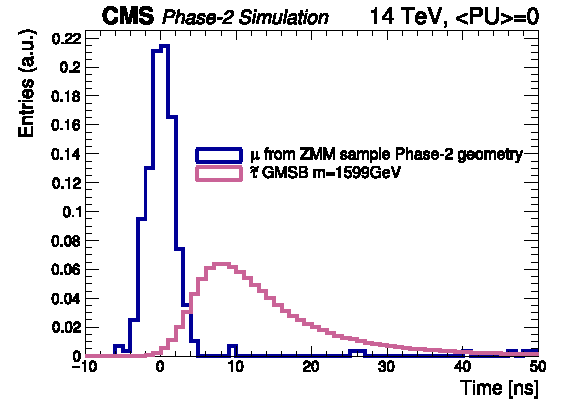
\includegraphics[width=\linewidth]{fig/chapt3/HSCP_Time_measurement.pdf}
		\caption{\label{fig:HSCP-Time} The measured transit time of a HSCP in CMS is compared to the transit time of a particle traveling at near the speed of light~\cite{PHASEIITP}.}
	\end{wrapfigure}
	
	Over its full lifetime, the HL-LHC is expected to deliver an outstanding integrated luminosity of \SI{3000}{fb^{-1}}, nearly an order of magnitude higher than what will be delivered by LHC until LS3 start, as shown in Figure~\ref{fig:HL-LHC-Timeline}. In the case of Higgs studies, this will lead to measuring the couplings of the boson to a precision of 2 to 5\%. Thanks to the estimated 15 millions of Higgs bosons created every year, a more precise measurement of potential deviations from the theoretical predictions is expected. The properties of the boson will hence be tested and compared to the SM Higgs neutral boson. SUSY and heavy gauge boson studies would also see their mass range limits pushed away by at least \SI{1}{TeV} and could lead to a new breakthrough. Many of the \acl{SM} extensions discussed in Section~\ref{chapt2:ssec:TeV} yield \acf{HSCPs}, i.e. heavy long-lived particles. These particles would be produced at the LHC with a high momentum but a velocity significantly lower than the speed of light ($\beta < 0.9$)~\cite{DREES1990,FAIRBAIRN2007,LIGETI2010,CMSHSCP2016,KHACHATRYAN2017} and/or a charge that differs from the elementary charge ($\vert Q \vert = e$, $\vert Q \vert < e$ or $\vert Q \vert > e$)~\cite{CMSHSCP2016,KHACHATRYAN2017,KUSENKO1998,KOCH2007,SCHWINGER1966,KHLOPOV2006}. Depending on the model considered, HSCPs could be lepton-like heavy particles or on the contrary R-hadron, i.e. particles composed of a supersymmetric particle and at least one quark~\cite{CMSHSCP2016}.
	
\endgroup

	\begin{figure}[H]
		\centering
		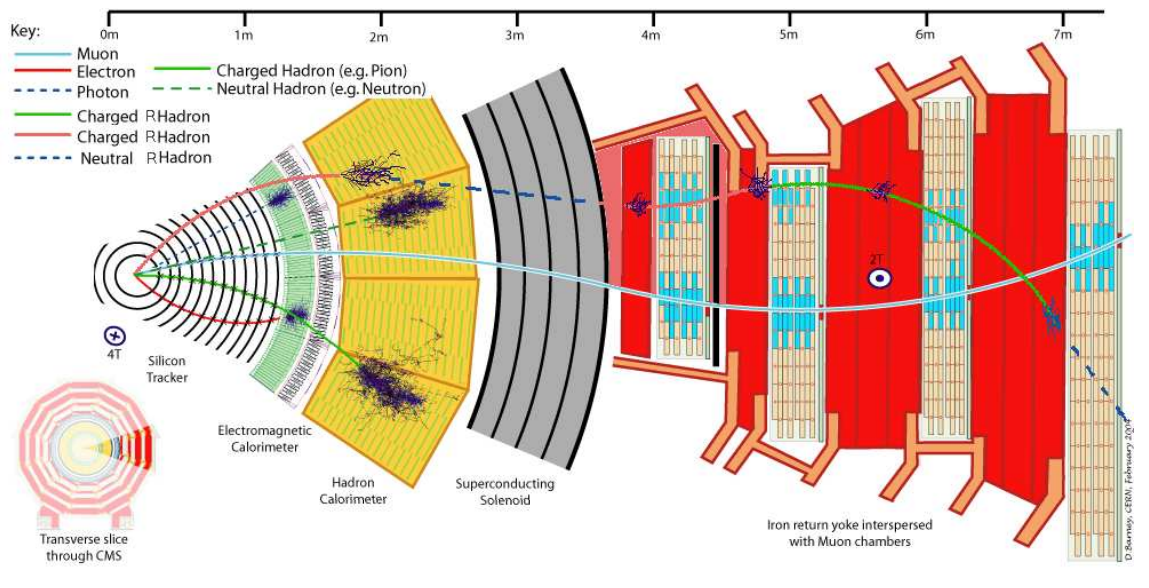
\includegraphics[height=7cm]{fig/chapt3/CMS-slice-HSCPs.png}
		\caption{\label{fig:HSCPs} Slice of the CMS detector showing example of passage of SM particles and R-hadrons. On the one hand, lepton-like HSCPs will appear to behave like slow and heavy muons. On the other hand, R-hadrons are likely to convert into other kind of charged or neutral R-hadrons due to interactions inside the detector volume.}
	\end{figure}
	
\begingroup\setlength{\intextsep}{5pt}\setlength{\columnsep}{15pt}
	
	\begin{wrapfigure}{r}{.5\linewidth}
		\centering
		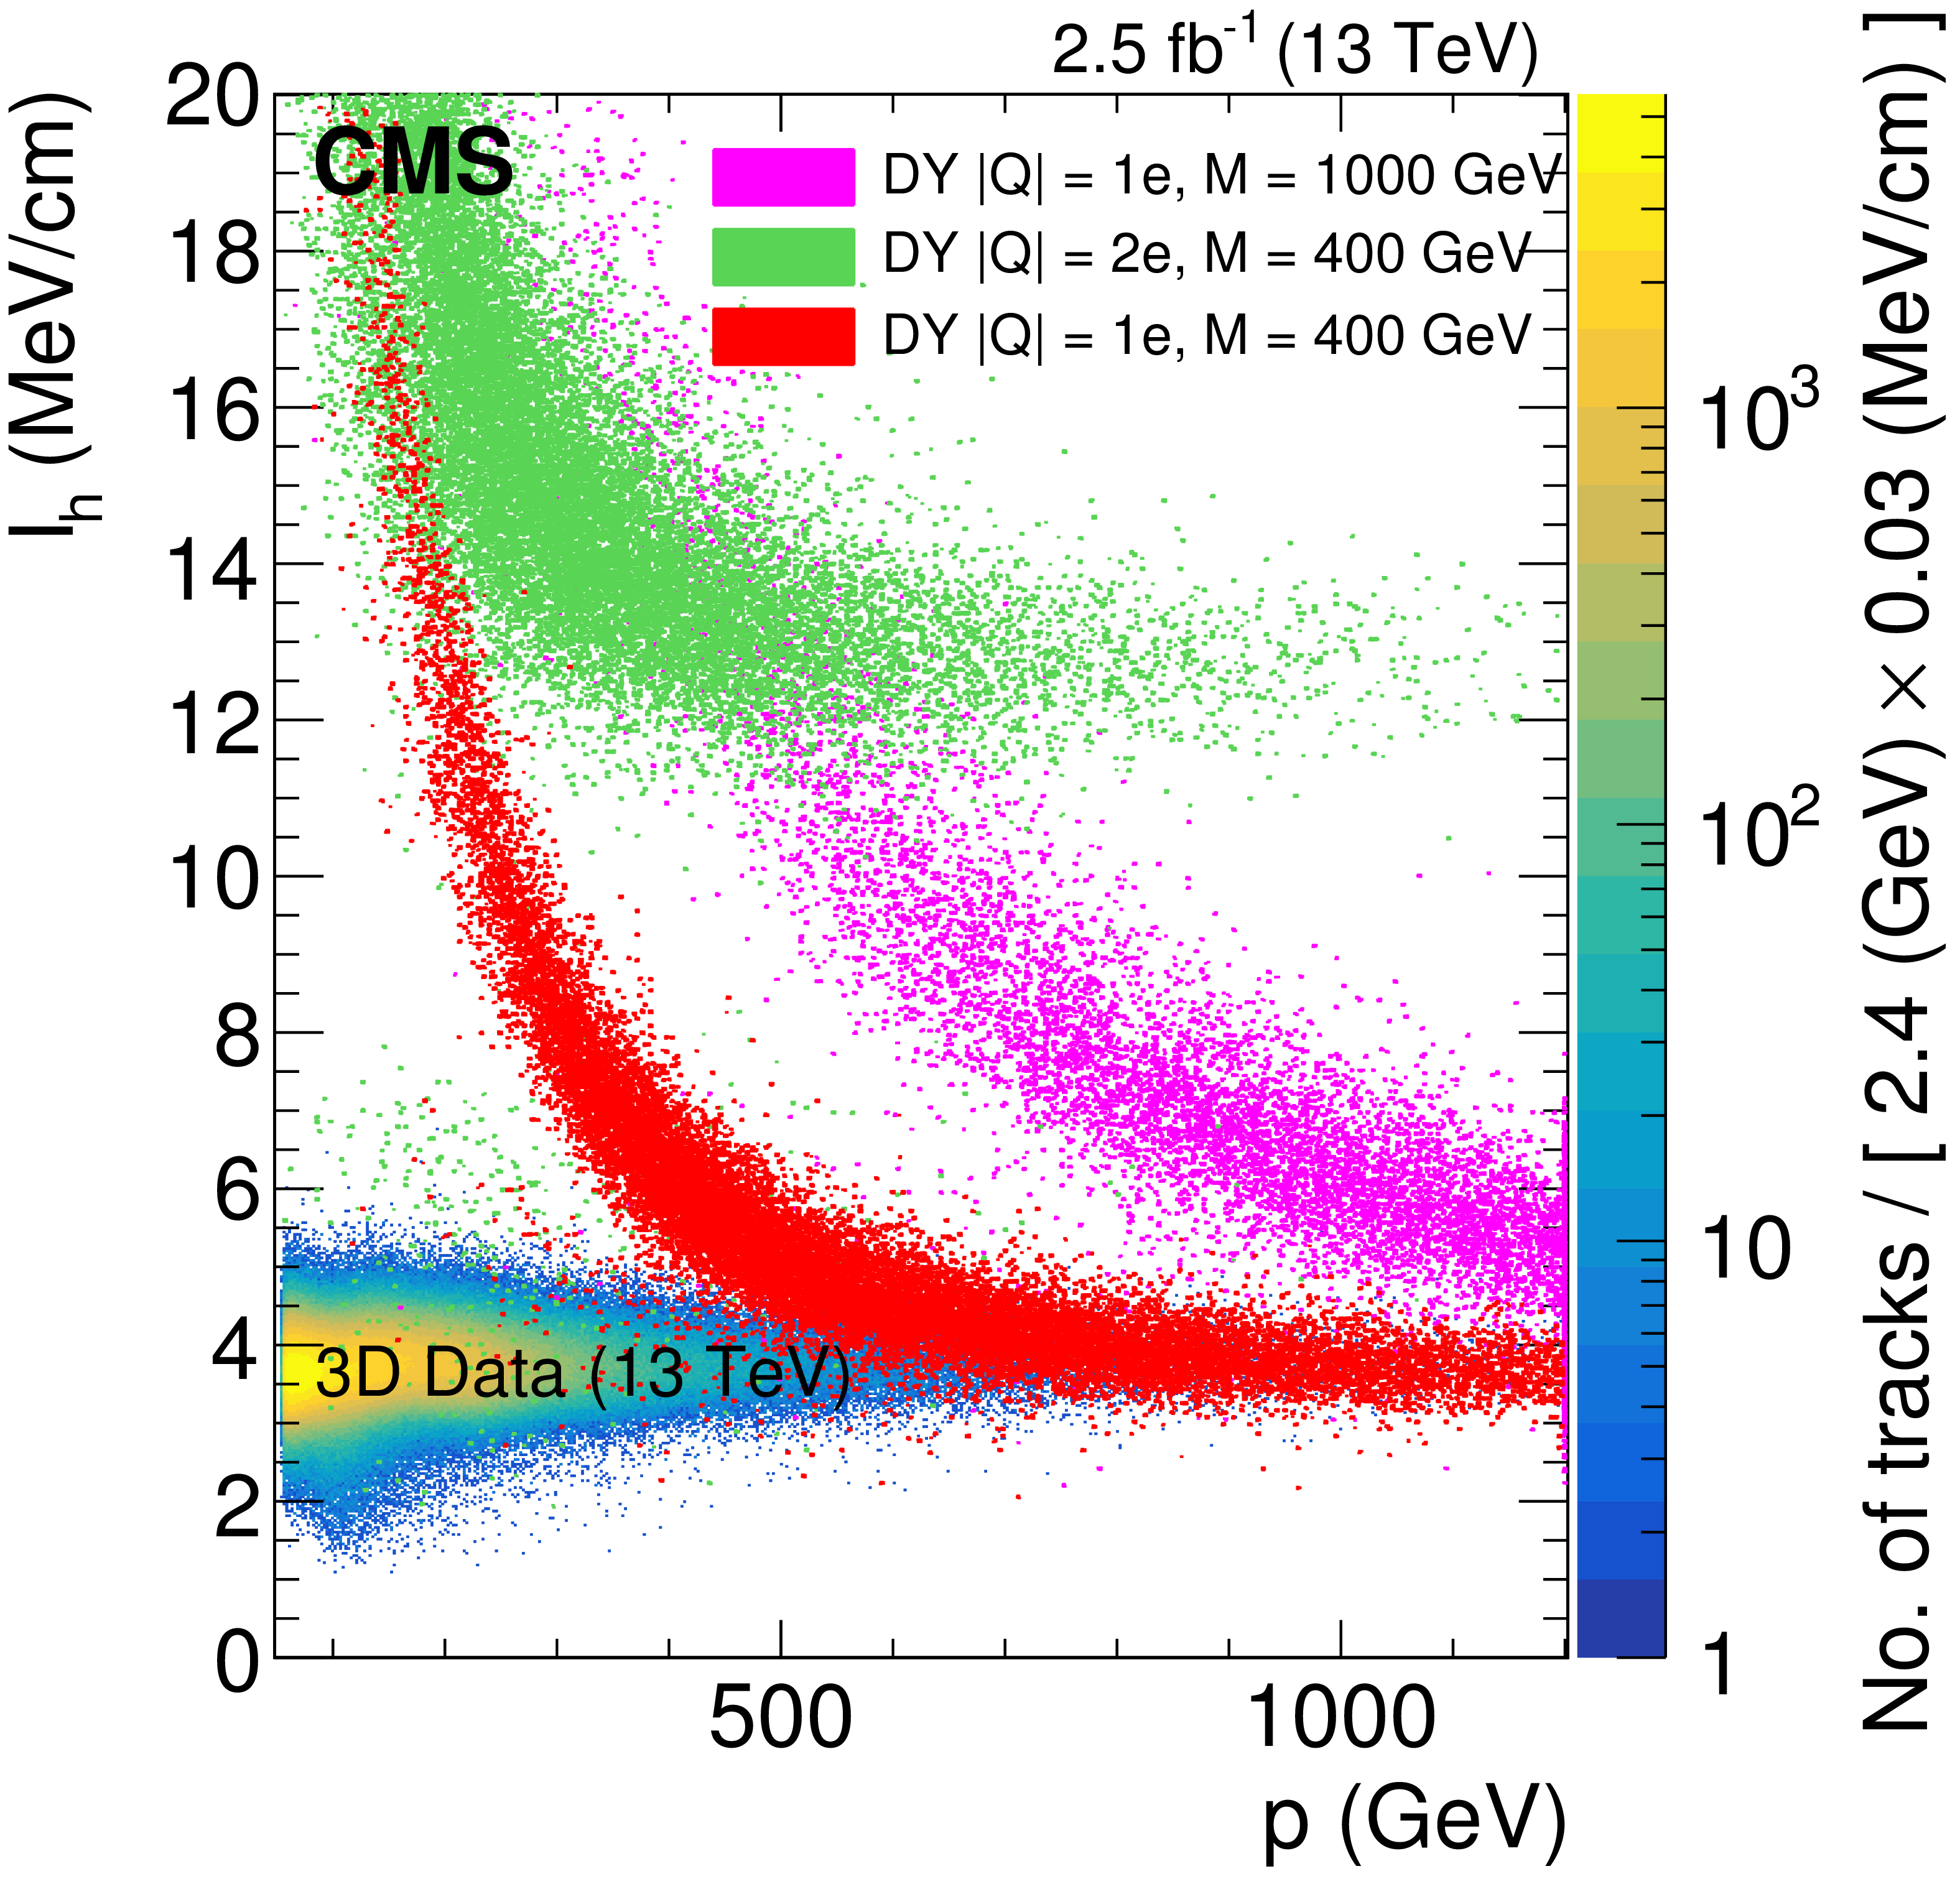
\includegraphics[width=\linewidth]{fig/chapt3/HSCPs_dEdx_CMS.png}
		\caption{\label{fig:dEdx-HSCPs} Distribution of the energy-loss $dE/dx$ as described by Bethe-Bloch formula through the estimator $I_h$ with increasing particle momentum for tracks in the \SI{13}{TeV} data. The estimator depends on the charge deposition of the particles per unit length in the silicon detectors of CMS which is related to their energy loss as explained in a publication by the CMS Collaboration~\cite{CMSHSCP2016}. The simulated HSCPs are singly or multiply charged particles with masses of 400 and \SI{1000}{GeV}.}
	\end{wrapfigure}
	
	Due to lifetimes of the order of a few \si{ns}, HSCPs would travel for long enough distances to cross through entire typical collider detectors while appearing almost stable. Because of their low velocity, they can be reconstructed and assigned to bunch crossings different to the ones they effectively have been produced, as shown in Figure~\ref{fig:HSCP-Time}, if reconstructed at all. Indeed, the trigger algorithms in use at CMS were not designed for such slow particles and they assume most particles of interest will have a velocity close to the speed of light~\cite{KHACHATRYAN2017,KAZANA2009}.
	
	As HSCPs are long-lived particles, their identification would be possible thanks to the muon system. The main background will consist of wrongly measured muons which should have a lower transverse momentum, a near to speed-of-light velocity and a low ionisation energy loss. An example of passage of HSCPs through a slice of the CMS detector is showed in Figure~\ref{fig:HSCPs}. The tracks associated to the HSCPs would then have to be reconstructed in both the silicon detectors, for precise $dE/dx$ measurement, and the muon system detectors. In this case, the muon system will be used to perform \acf{ToF} measurements to discriminate between near spead-of-light particles and slower ones. The full reconstruction will then look for useful signatures such as the large transverse momentum of the candidates or their large ionisation energy loss alongside the low velocity accurately measured thanks to the muon system as depicted in Figure~\ref{fig:dEdx-HSCPs}. The ToF measurement to identify beyond the \acl{SM} particles will mostly rely on the time information provided by the \acl{DT}s, in the barrel region of the detector, and \acl{CSC}s, in the endcaps. From CMS point of view it will then become necessary to increase the acceptance and redundancy of the endcaps toward higher pseudo-rapiditiy as the pseudo-rapidity region \psrapr{1.6}{2.5} is only covered by CSCs.\\
	
\endgroup

	A natural consequence of the higher instantaneous luminosity will be the increase of collisions per bunch crossing. It is estimated that the \acl{PU} will rise from the approximate average of 40 collisions per bunch crossing in 2017 and 2018, presented in Figure~\ref{fig:CMS-pileup}, to 140 to 200 depending on the scenario considered~\cite{MEDINAMEDRANO2017}. The trigger rate will then be affected in the same way putting a lot of stress on the trigger algorithms. Upgrading the electronics of some of the detectors and working on the data flow within the experiment would help going through HL-LHC with keeping similar performance than during Phase-1. On the other hand, the impact of the increased background will become problematic in many ways and will force for upgrades or many sub-systems of CMS. The main effects will be a large increase of the irradiation of the detectors, mainly close to the beam line. The detectors already installed will need to be certified for the irradiation levels they will be subjected to until the end of HL-LHC while the new detectors that will extend the coverage of the muon system toward higher pseudo-rapidity will need to take the strong radiations they will suffer close to the beam line into account. Simulations of the expected distribution of absorbed dose in the CMS detector under HL-LHC conditions show, in Figure~\ref{fig:Dose}, that detectors placed close to the beam line will have to withstand high irradiation, the radiation dose being of the order of a few tens of \si{Gy}.
	
\begingroup\setlength{\intextsep}{5pt}\setlength{\columnsep}{15pt}

	\begin{wrapfigure}{L}{.6\linewidth}
		\centering
		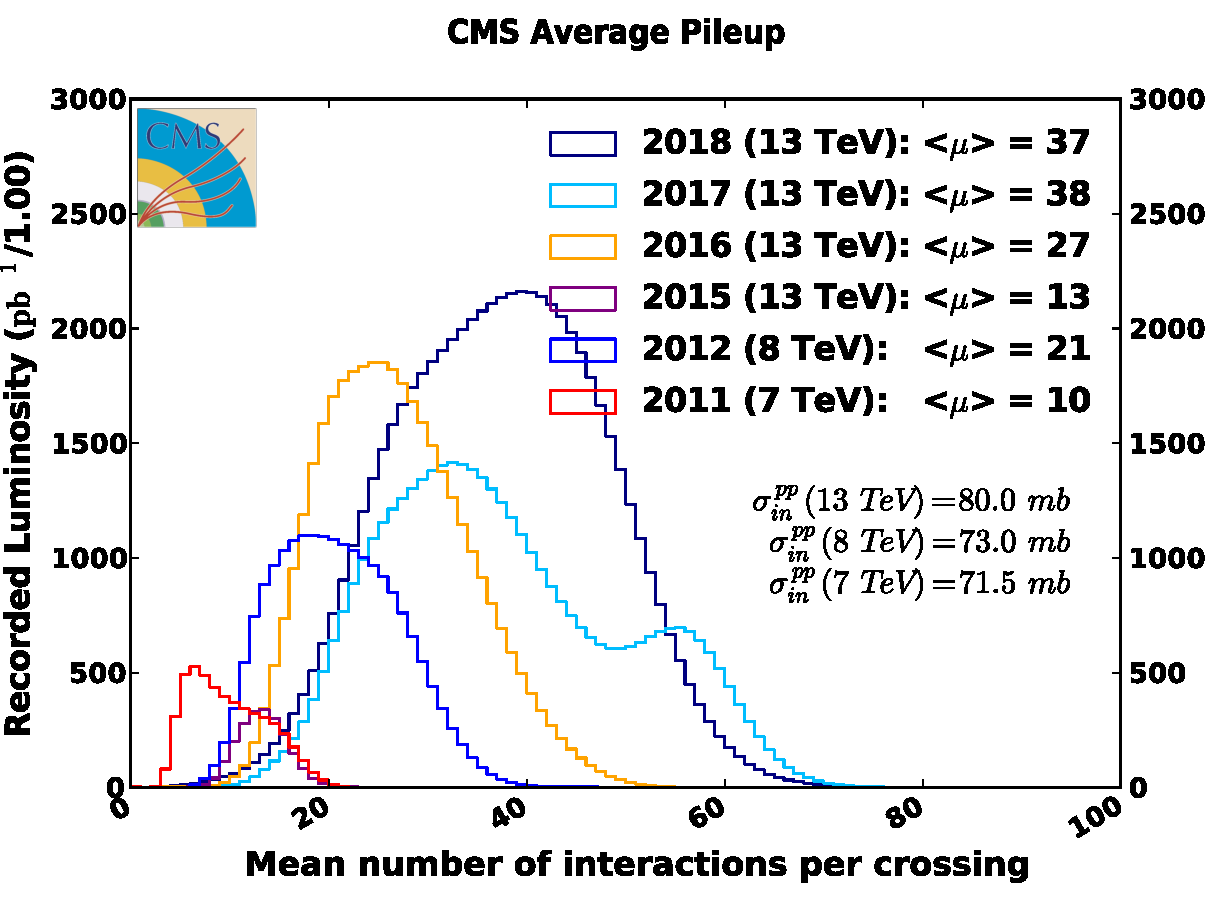
\includegraphics[width=\linewidth]{fig/chapt3/CMS_pileup_pp_2018.pdf}
		\caption{\label{fig:CMS-pileup} Distribution of the average number of interactions per crossing (pileup) for pp collisions in 2011 (red), 2012 (blue), 2015 (purple), 2016 (orange), 2017 (light blue), and 2018 (navy blue). The overall mean values and the minimum bias cross sections are also shown~\cite{LUMIPUBLICCMS}.}
	\end{wrapfigure}

	Improving this situation will come with the increase of hit numbers recorded along the particle track to reduce the ambiguity on muon versus background detection. Moreover, the measurement of small production cross-section and/or decay branching ratio processes, such as the Higgs boson coupling to charge leptons, and in particular to muons, or the $B_s \rightarrow \mu^+\mu^-$ decay, is of major interest. Such sonsiderations give more weight to the upgrade of the forward regions to maximize the physics acceptance to the largest possible solid angle.
	
\endgroup
\begingroup\setlength{\intextsep}{5pt}\setlength{\columnsep}{15pt}

	\begin{wrapfigure}{L}{.6\linewidth}
		\centering
		\vspace{25pt}
		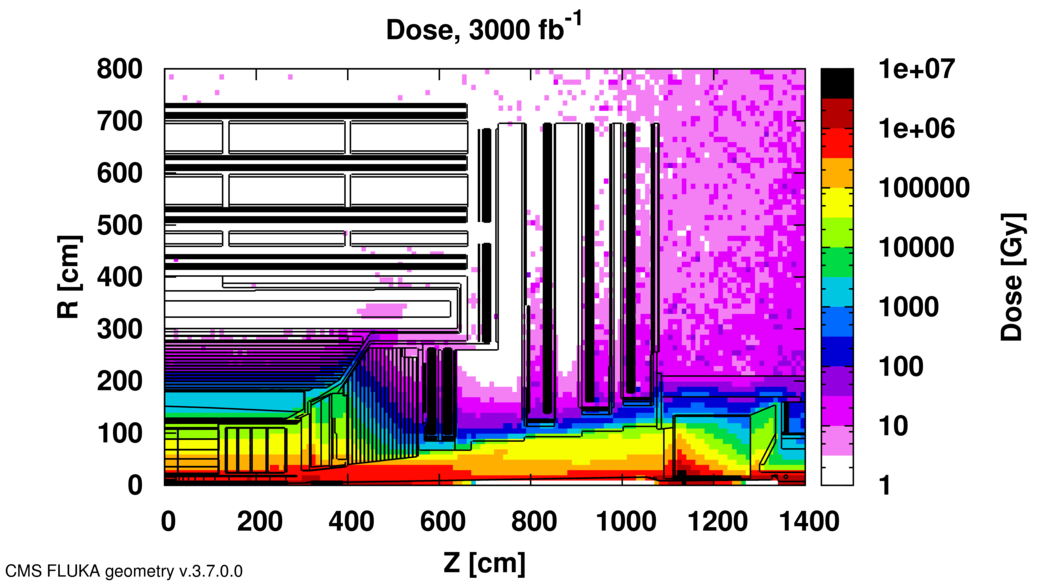
\includegraphics[width=\linewidth]{fig/chapt3/HL-LHC-Dose.png}
		\caption{\label{fig:Dose} Absorbed dose in the CMS cavern after an integrated luminosity of \SI{3000}{fb^{-1}}. Using the interaction point as reference, R is the transverse distance from the beamline and Z is the distance along the beamline~\cite{PHASEIITP}.}
	\end{wrapfigure}
	
	To ensure proper trigger performance within the present coverage, the muon system will be completed with new chambers and the electronics of the present system will need to be upgraded. A first step into this direction will be taken by installing new gaseous detectors in each endcap layers and extend the coverage up to \psrape{2.8}. Nevertheless, the region beyond \psrapg{2.8} and extending to \psrape{5.0} only is covered by the forward HCAL detectors and lack redundant muon detector coverage. Extensions of the tracker in the context of HL-LHC will increase its coverage up to \psrape{4.0} but the identification of muons and measurement of their energy with reasonable precision only using the tracker is nearly impossible. Thus, this increased tracker coverage range needs to be put in parallel with a matching muon detector and will open doors to multi-lepton final states in which leptons are likely to have a a low transverse momentum and to be found near the beam line.
	
	Finally, as the muon system is composed only of gaseous detectors, strong environmental concerns have risen over the last years as the European directives will restrict the use of fluorine based gas mixtures. Both the CSC and RPC subsystems, using $CF_4$, $C_2H_2F_4$, or $SF_6$, will need to adapt their working gas in order to strongly reduce the greenhouse potential of the mixtures released into the atmosphere due to gas leaks.
	
\endgroup
	
\section{Desciption of the muon system}
\label{chapt3:sec:muonsystem}
	
	\begin{figure}[H]
		\begin{subfigure}{0.35\linewidth}
			\centering
			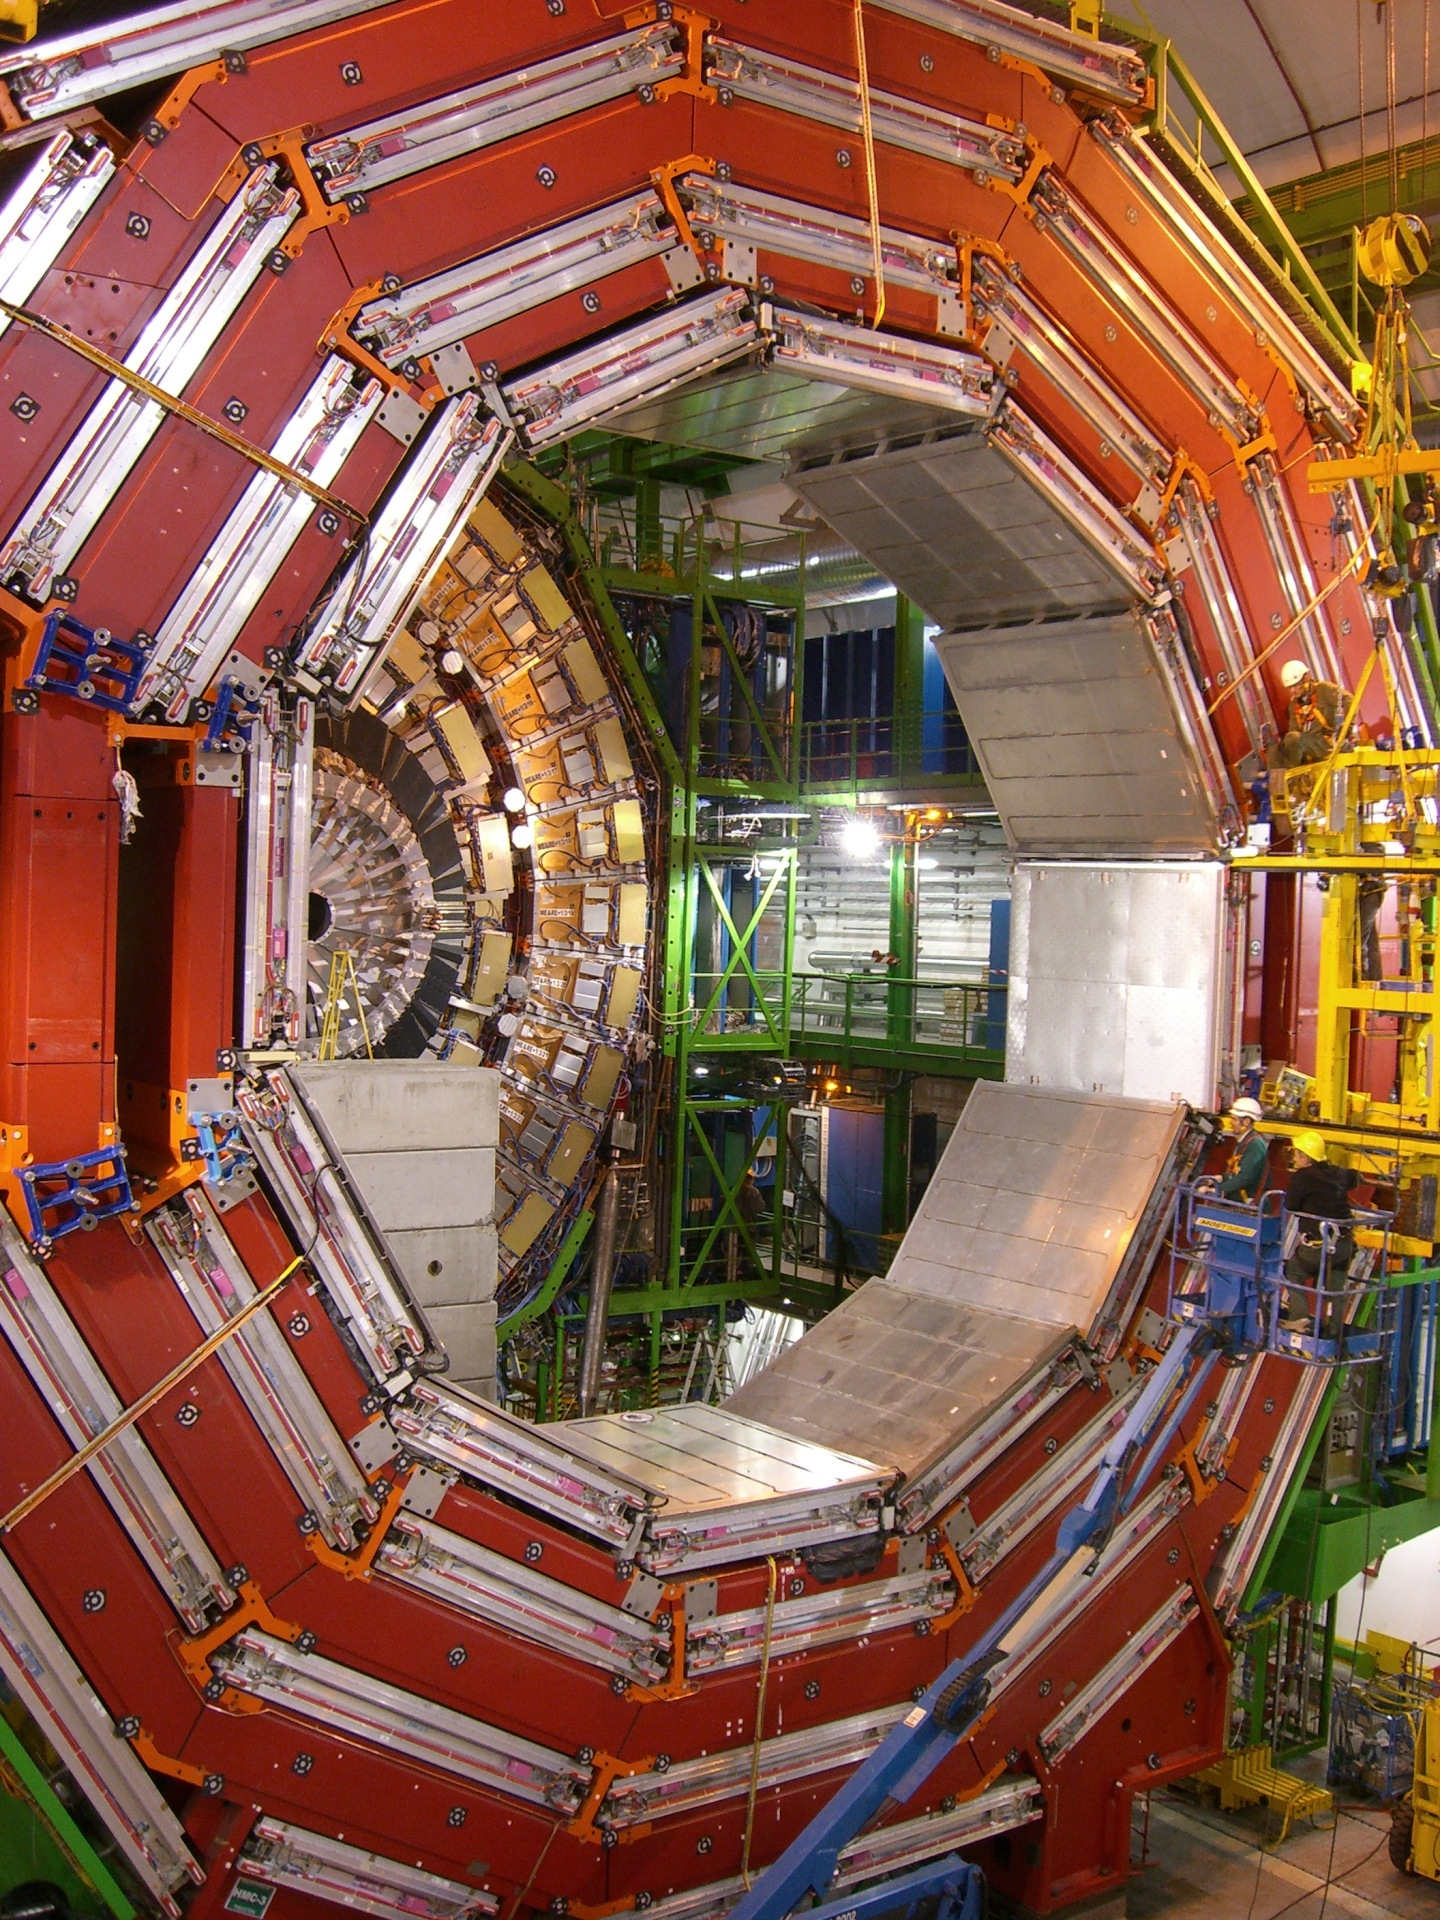
\includegraphics[height = 6cm]{fig/chapt3/Wheel.jpg}
			\caption{\label{fig:Muon:A}}
		\end{subfigure}
		\begin{subfigure}{0.3\linewidth}
			\centering
			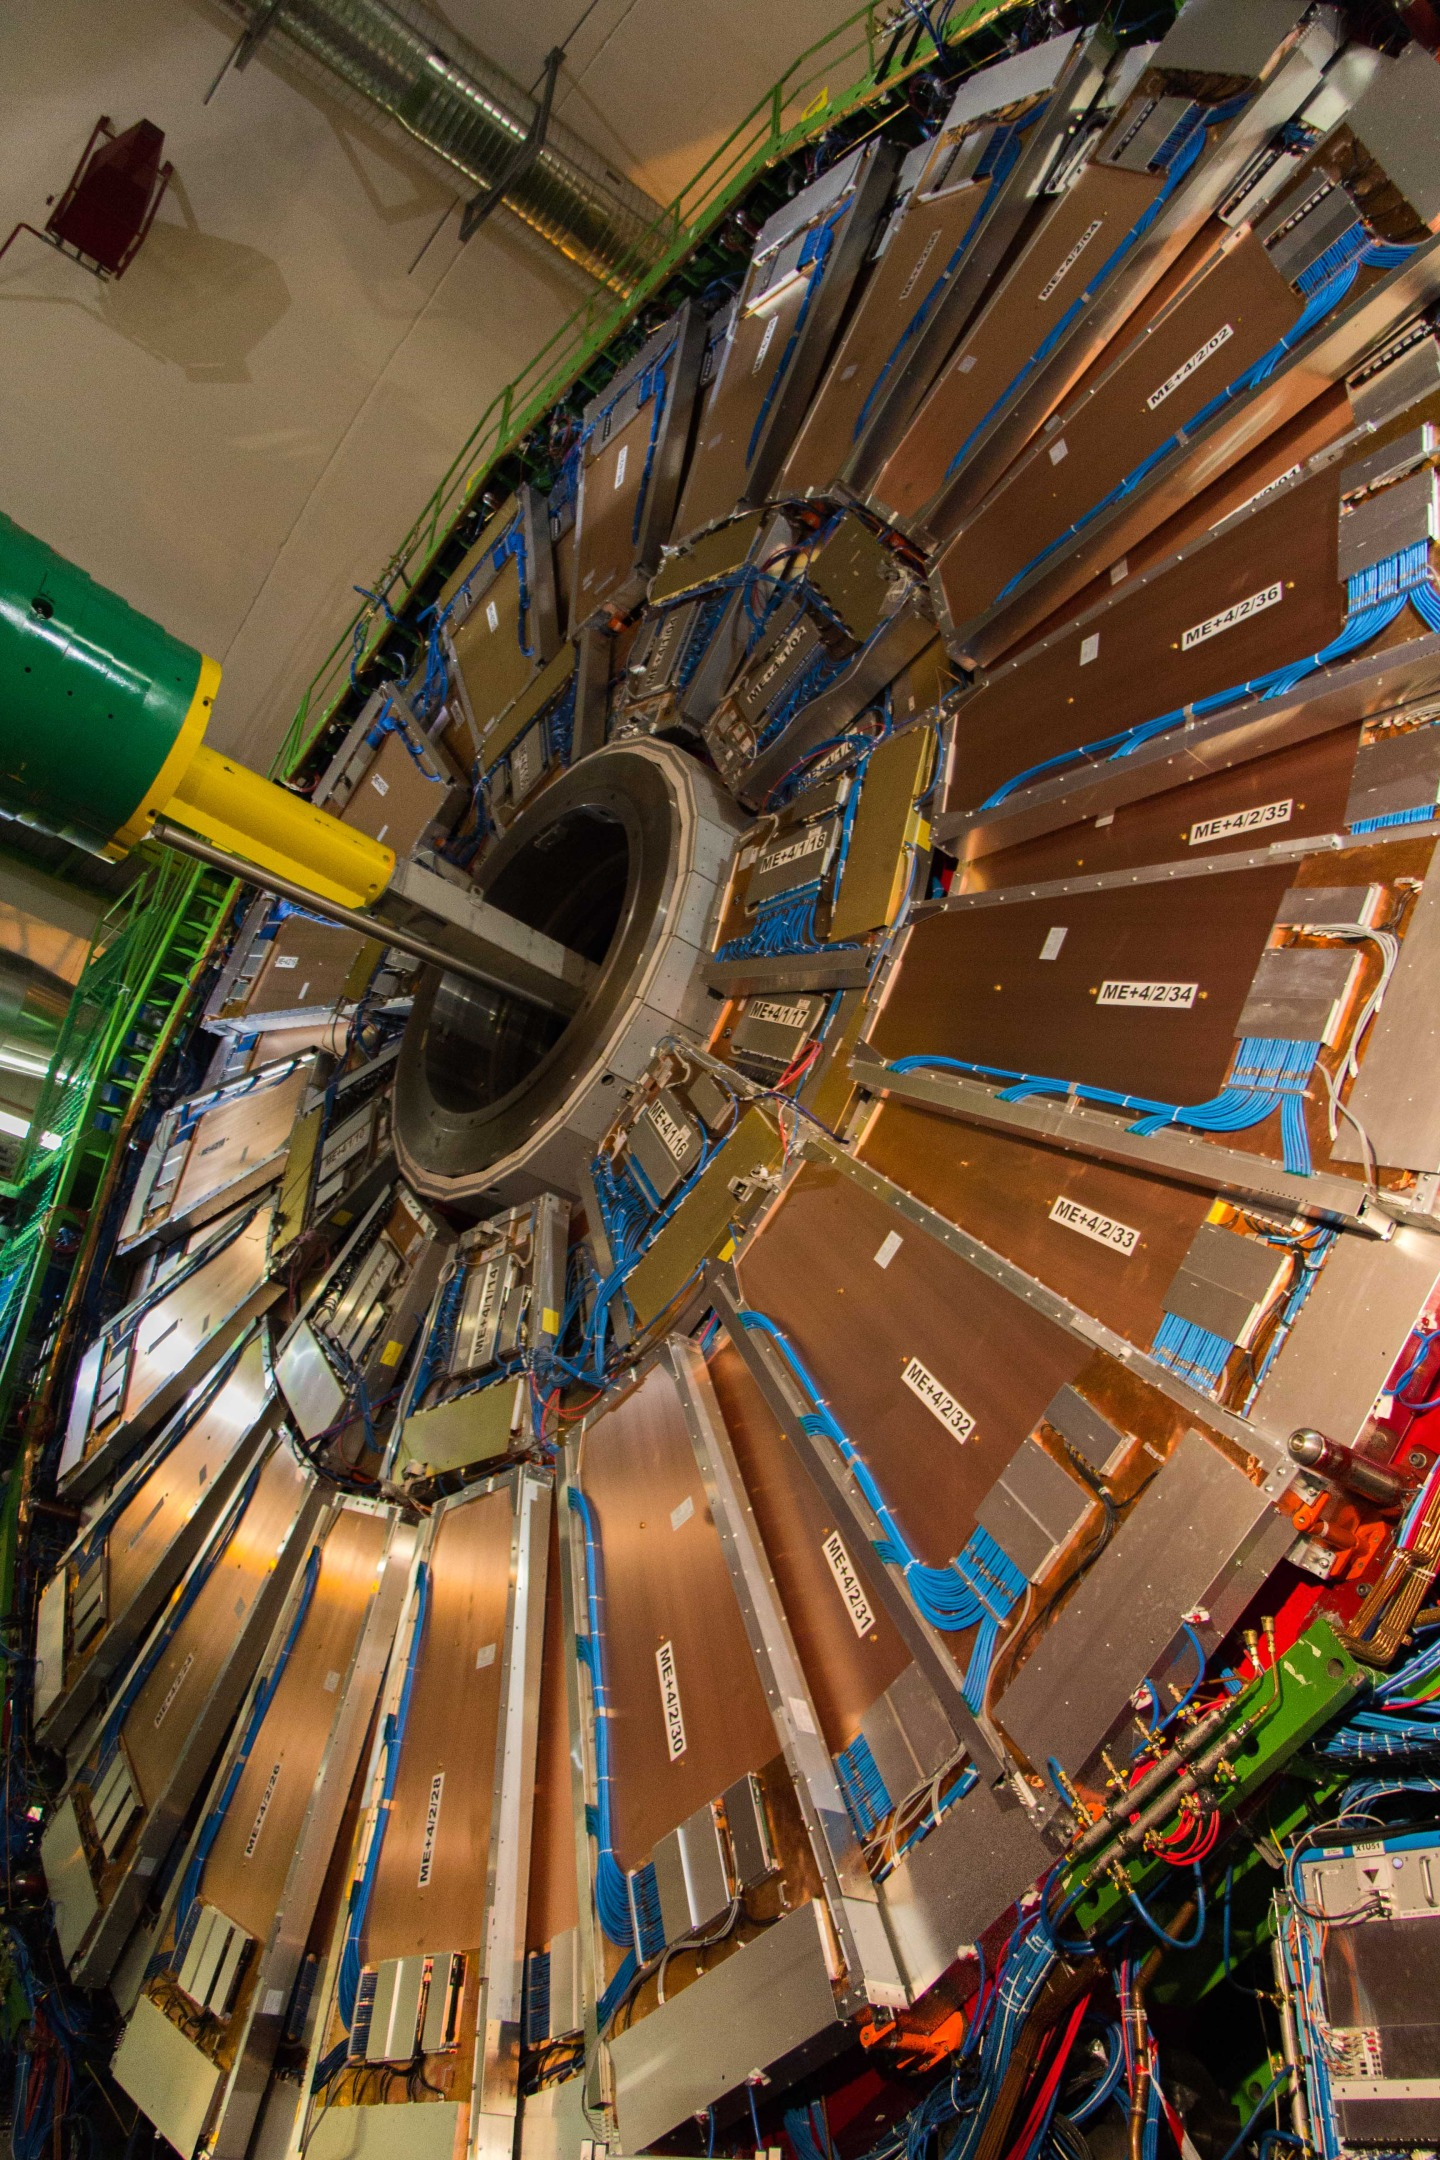
\includegraphics[height = 6cm]{fig/chapt3/Disk_CSC.jpg}
			\caption{\label{fig:Muon:B}}
		\end{subfigure}
		\begin{subfigure}{0.35\linewidth}
			\centering
			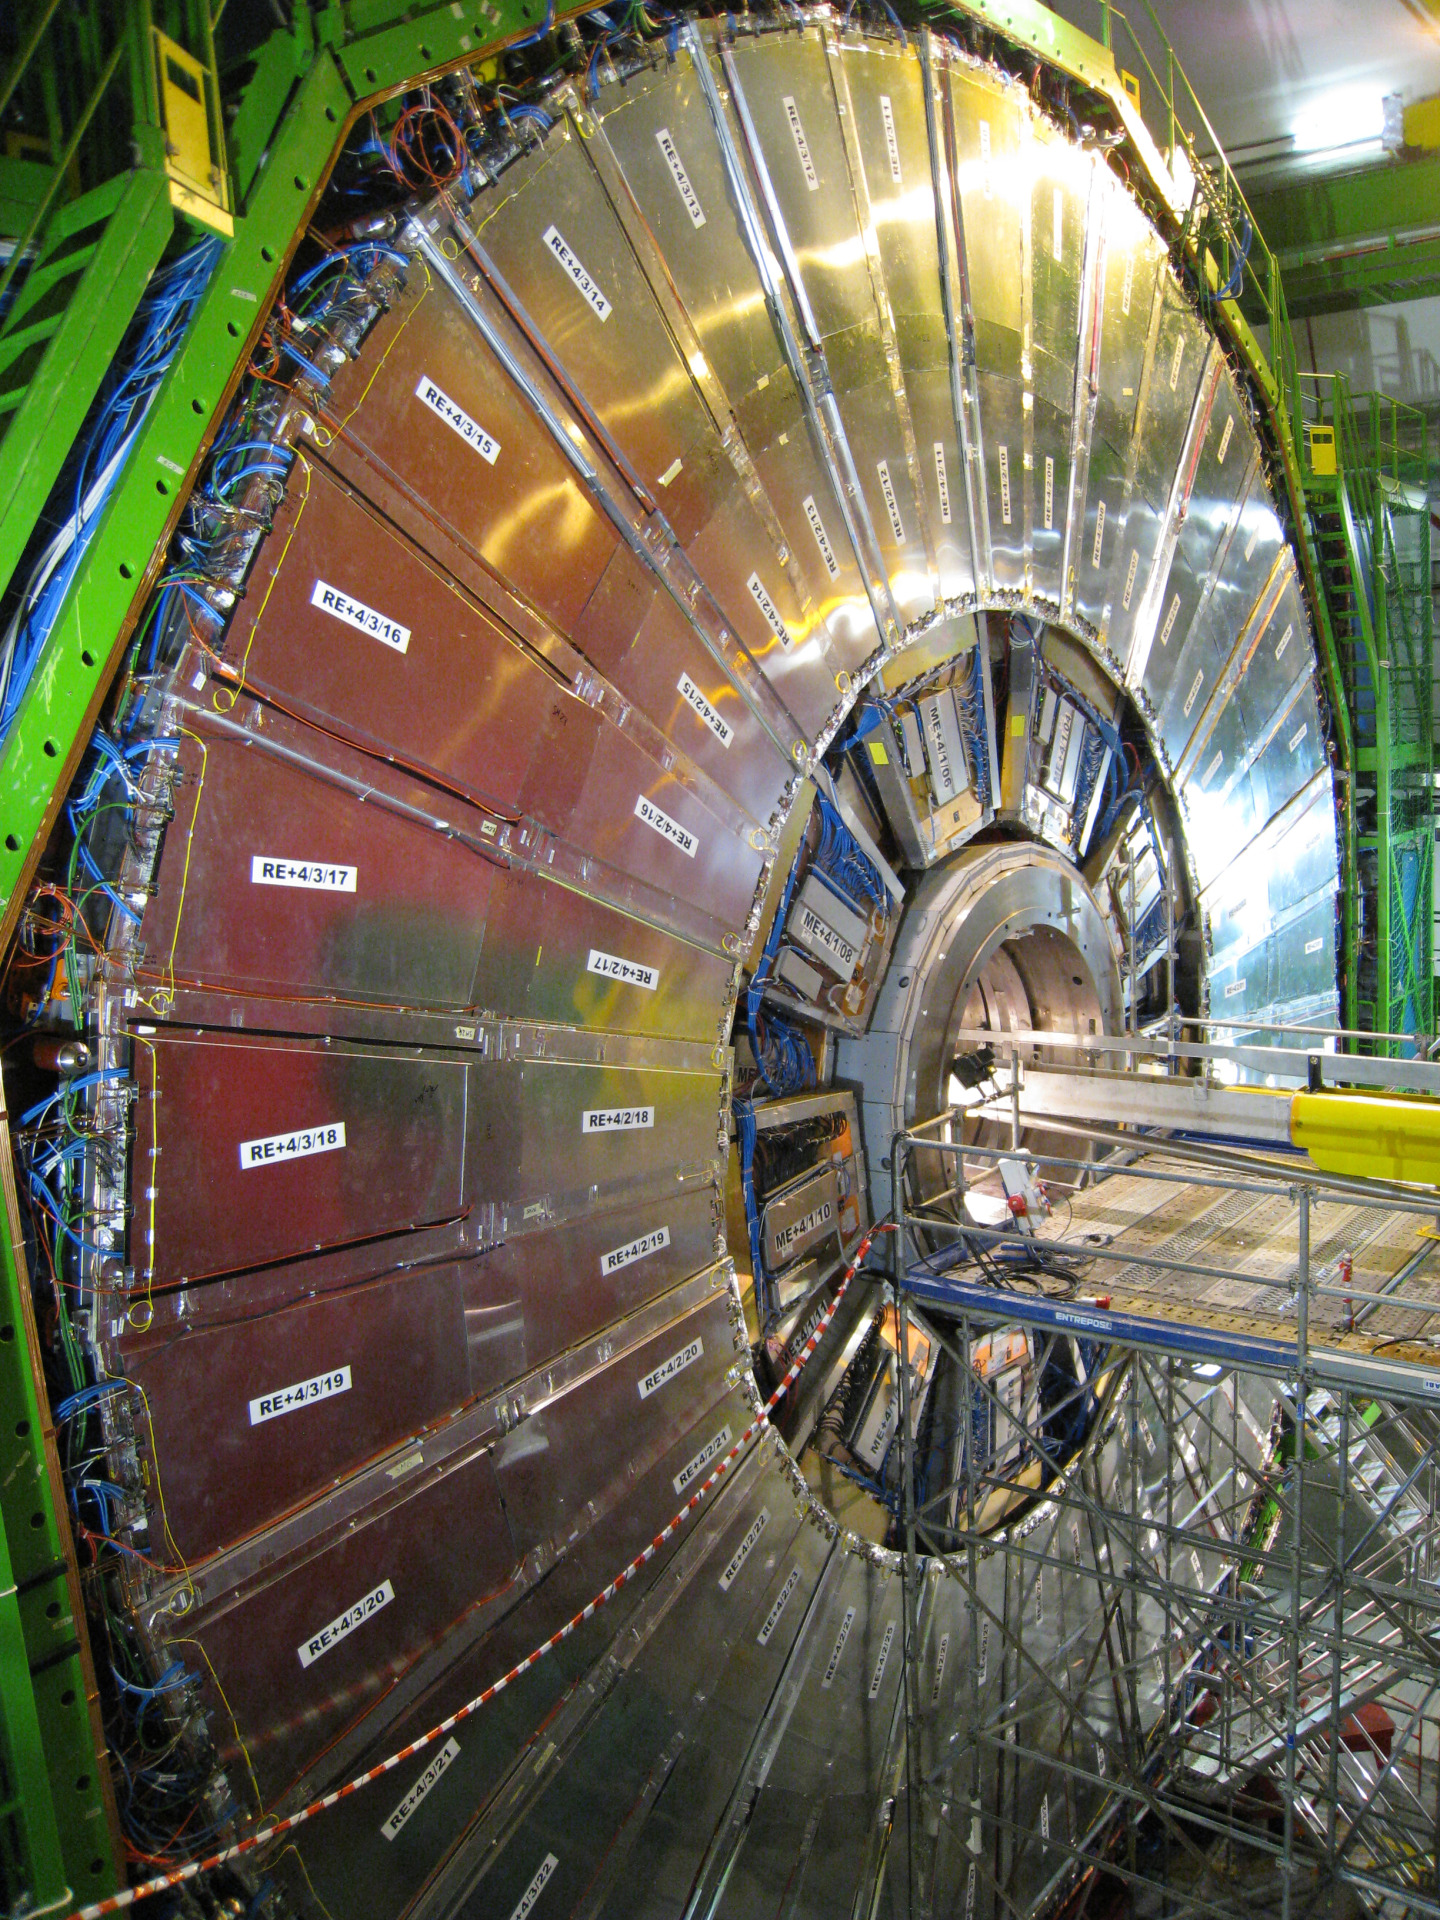
\includegraphics[height = 6cm]{fig/chapt3/Disk_RPC.jpg}
			\caption{\label{fig:Muon:C}}
		\end{subfigure}
		\caption{\label{fig:Muon} Figure~\ref{fig:Muon:A}: Barrel wheel with its detector rings and return yokes. Figure~\ref{fig:Muon:B}: CSC endcap disk with the 2 CSC stations. The outer station is made of \SI{10}{\deg} detectors while the inner station is made of \SI{20}{\deg} detectors. Figure~\ref{fig:Muon:C}: RPC endcap disk. The inner station is not equipped and the inner CSC station can be seen.}
	\end{figure}
	
	The barrel region is divided into 5 \textit{wheels} made out of 4 \textit{rings} of detectors with iron return yokes in between them whereas the endcaps are made out of 4 disks, each divided into pseudorapidity stations, 2 for CSCs (except for the first disk where 3 stations are equipped) and 3 for RPCs, although only 2 RPCs stations are equipped at present. The wheels and disks are shown in Figure~\ref{fig:Muon}. So far, each subsystem was dedicated to a particular task. DTs, in the barrel, and CSCs, in the endcaps, are used mainly for their spatial resolution. Indeed, DTs' resolution is of the order of \SI{100}{\micro m} along both the $(r-\phi)$ and $(r-z)$ components while the resolution of CSCs is similar but varies in a range from \SI{50}{\micro m} to \SI{140}{\micro m} depending on the distance to the beamline. On the other hand, RPCs are used as redundant detection system in the whole muon system. They display a very good intrinsic time resolution of \SI{1.5}{ns} although the electronics only provide bunch crossing information with a time resolution of \SI{25}{ns}.
	
	\subsection{The \acl{DT}s}
	\label{chapt3:ssec:DTs}
	
	The 250 CMS DTs, found in the barrel covering the pseudorapidity region \psrapr{0}{1.2} and whose structure is shown in Figure~\ref{fig:DT}, are composed of 3 \textit{superlayers} of DT cells. Two of these superlayers are dedicated to measuring the $\phi$ coordinate of the muons and while the last one measures the $\eta$ (or $z$) coordinate. Each superlayer consists on 4 layers of 60 to 70 DT cells arranged in quincunx to allow for a precise reconstruction of the muon path through the DT layers. Each DT cell is a rectangular aluminium gas volume with a central anode wire. Cathode strips are placed on the narrow surface of the cells and electrode strips are placed on the wide surface to help shaping the electric field to ensure a consistent drift velocity of electrons in the drift volume. These detectors are operated using a 85/15 mixture of $Ar$ and $CO_2$. Outside the gas volume of each DT chamber is attached a \acf{MiC} that hosts both read-out and trigger electronics.
	
	\begin{figure}[H]
		\begin{subfigure}{0.6\linewidth}
			\centering
			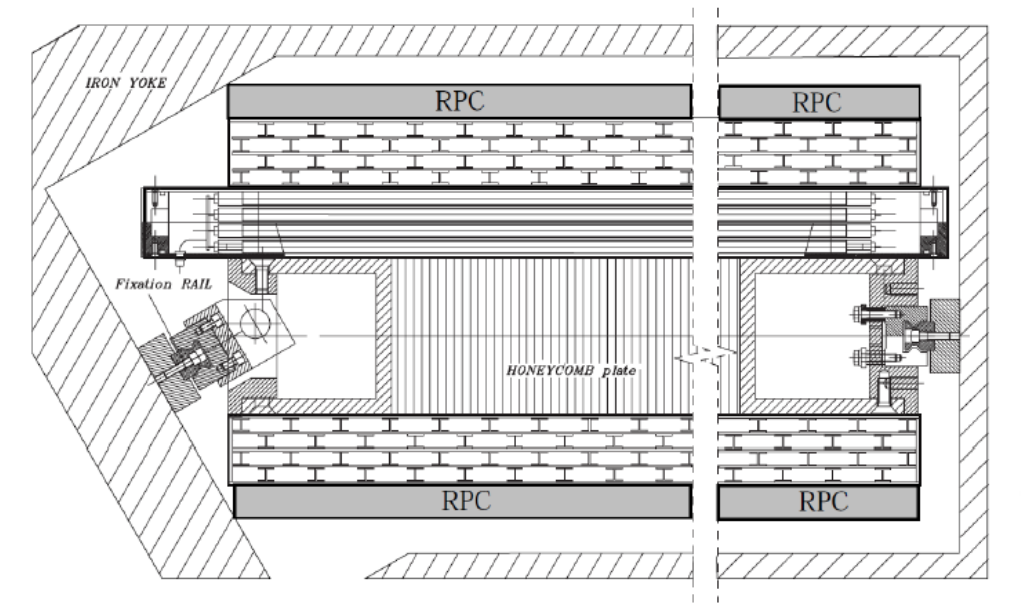
\includegraphics[height = 4.5cm]{fig/chapt3/DT_layout.png}
			\caption{\label{fig:DT:A}}
		\end{subfigure}
		\begin{subfigure}{0.4\linewidth}
			\centering
			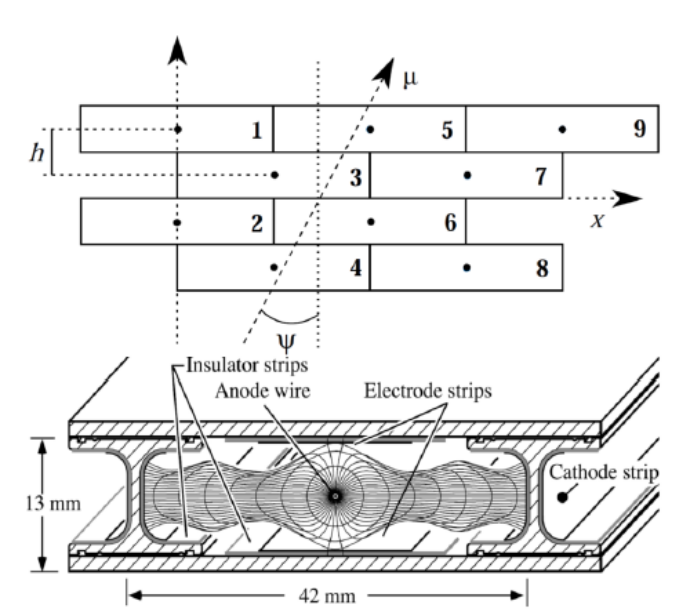
\includegraphics[height = 4.5cm]{fig/chapt3/DT_cells.png}
			\caption{\label{fig:DT:B}}
		\end{subfigure}
		\caption{\label{fig:DT} Figure~\ref{fig:DT:A}: Cross section of a DT module showing the two superlayers measuring the $\phi$ coordinate, perpendicular to the cross section plane, and the superlayer measuring the $\eta$ coordinate, placed in between the two others with honeycomb and parallel to the cross section plane. The DT detector is sandwiched in between 2 RPCs whose readout strips are perpendicular to the cross section plane, measuring the $\phi$ coordinate. Figure~\ref{fig:DT:B}: A DT cell is shown together with its electric field. The path of a muon through a superlayer is shown.}
	\end{figure}
	
	\subsection{The \acl{CSC}s}
	\label{chapt3:ssec:CSCs}
	
	The 540 CMS CSCs, found in the endcaps covering the pseudorapidity region \psrapr{0.9}{2.5} and described through Figures~\ref{fig:CSC-layout} and \ref{fig:CSC-track}, are composed of 6 panels of CSC, each panel consisting in a wide gas volume of \SI{9.5}{mm} (\SI{7}{mm} in the case of ME1/1 station) containing anode wires and whose surfaces are cathodes. The top cathode is a wide copper plane of the size of the gas volume. The bottom cathode is divided into thin trapezoidal copper strips radially arranged to measure the azimuthal coordinate $\phi$ with a pitch ranging from 8 to \SI{16}{mm}. The \SI{0.50}{\micro m} anode wires are placed perpendicularly to the strips to measure radial coordinate $r$ and are grouped by 10 to 15 with a wire to wire space of \SI{3.2}{mm}. In he specific case of ME1/1 placed against the HCAL endcap, the \SI{0.30}{\micro m} anode wires have a wire to wire distance of \SI{2.5}{mm} and are not disposed perpendicularly to the strips but slightly tilted by an angle of \SI{29}{\deg} to compensate for the lorentz force due to the very strong local magnetic field of \SI{4}{T}. These detectors are operated with a 40/50/10 mixture of $Ar$, $CO_2$ and $CF_4$. Combining the information of the multiple CSC panels, the detectors achieve a very precise measurement of the muon track. The read-out of the cathode strip signals is performed by \acf{CFEBs} mounted on the detectors. The boards are used to collect and digitize the charge of the singals and transfer it to off-chamber electronics called \acf{DMBs}. In parallel, the data from the CFEBs together with the data from the anode wires, after treatment by on-chamber electronics called \acf{ALCTs}, is used to build a fast trigger information which is sent other off-chamber electronics called \acf{TMBs}.
	
	\begin{figure}[H]
		\begin{subfigure}{0.4\linewidth}
			\centering
			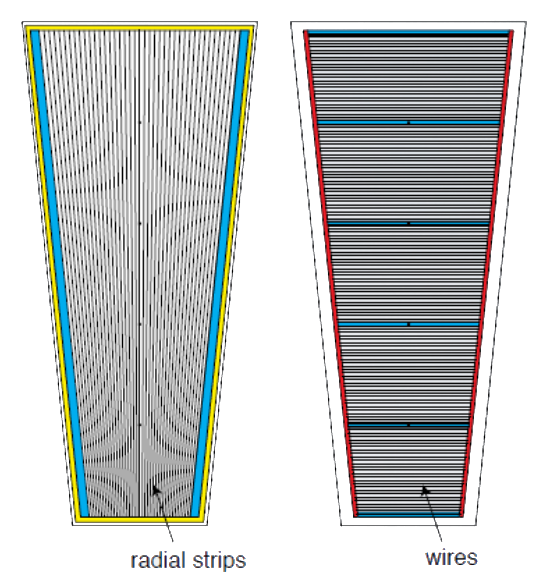
\includegraphics[height = 5cm]{fig/chapt3/CSC_layout.png}
			\caption{\label{fig:CSC-layout:A}}
		\end{subfigure}
		\begin{subfigure}{0.6\linewidth}
			\centering
			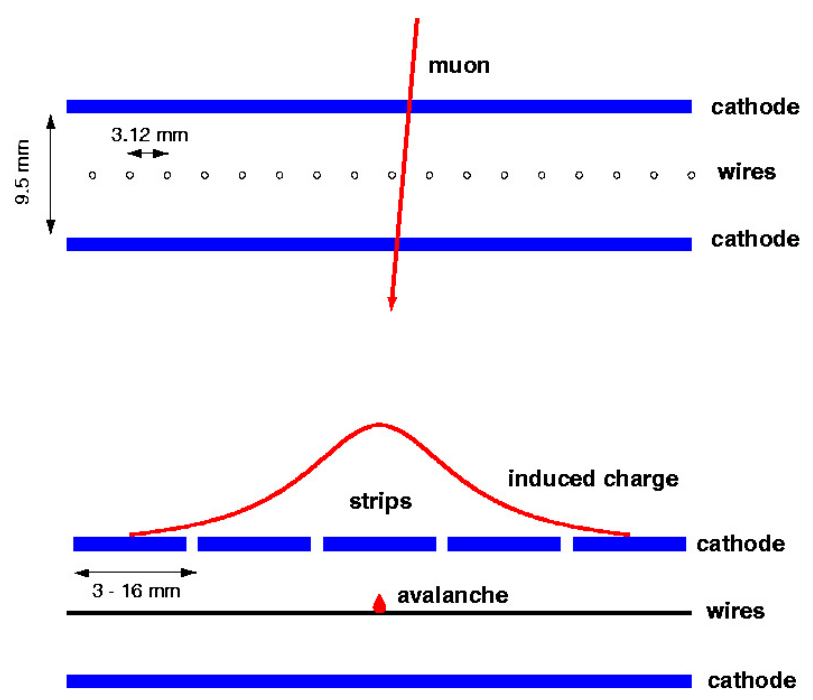
\includegraphics[height = 5cm]{fig/chapt3/CSC_avalanche.png}
			\caption{\label{fig:CSC-layout:B}}
		\end{subfigure}
		\caption{\label{fig:CSC-layout} Figure~\ref{fig:CSC-layout:A}: Cathode strips and anode wire layout of a CSC panel. Figure~\ref{fig:CSC-layout:B}: Avalanche development and charge collection by anode wires and induction on cathode strips inside of a CSC panel.}
	\end{figure}
	
	\begin{figure}[H]
		\centering
		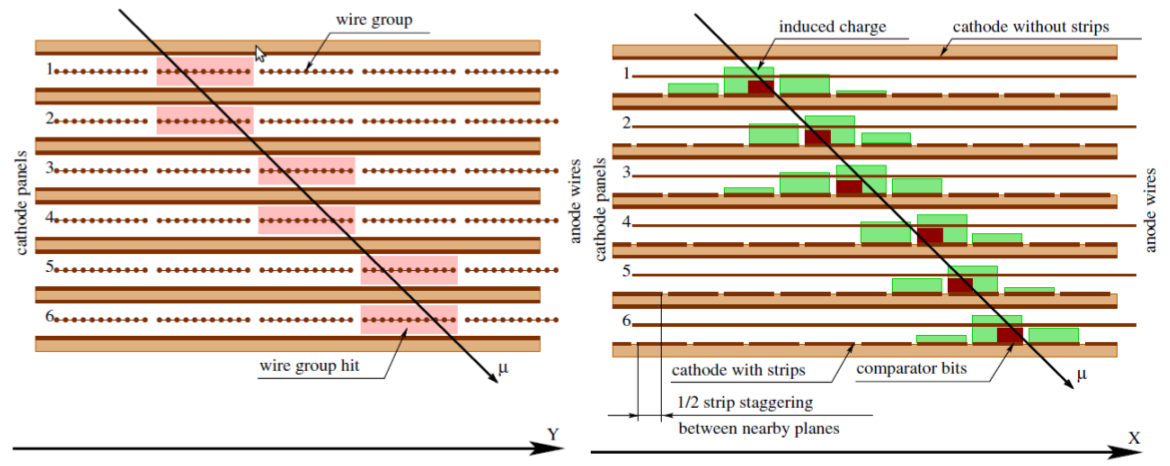
\includegraphics[width=\linewidth]{fig/chapt3/CSC_track.png}
		\caption{\label{fig:CSC-track} Muon track reconstruction through the 6 panels of a CMS CSC using the information of anode wire groups and cathode strip charge distribution combined with comparator bits to decide on which half strip the muon is more likely to have passed.}
	\end{figure}
	
	\subsection{The \acl{RPC}s}
	\label{chapt3:ssec:RPCs}
	
	Despite their excellent spatial resolution, the wire chambers (DTs and CSCs) are limited in terms of time resolution by the fact that the charge needs to drift towards the anode wire and be collected before having the confirmation that a particle was detected as the drift volume is not used to develop avalanches. Indeed, the stronger electric field close to the anode wire triggers the avalanche and the gain of the detector. Due to the drift, the time resolution is thus limited at best to approximately 2 to \SI{3}{ns}. In addition, even though the intrinsic time resolution of the tracking chambers is rather good compared to the \SI{25}{ns} in between successive collisions, the processing time of the trigger system doesn't allow for very fast triggering as it provides a time precision of only \SI{12.5}{ns}. Thus, detectors fully dedicated to timing measurement have been installed as a redundant system. These detectors are RPCs, also gaseous detectors but that use current induction instead of charge collection allowing for a time resolution of the order of \SI{1}{ns} only. Theoretically, depending on the design used, RPCs could reach a time resolution of the order of \SI{10}{ps} but in the context of LHC where bunch crossing happen every \SI{25}{ns}, a time resolution of \SI{1}{ns} is sufficient to accurately assign the right bunch crossing to each detected muon.
\begingroup\setlength{\intextsep}{5pt}\setlength{\columnsep}{15pt}

	\begin{wrapfigure}{r}{.65\linewidth}
		\centering
		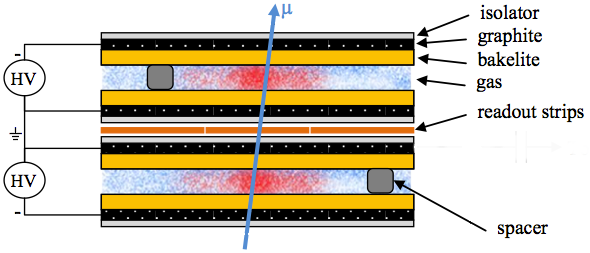
\includegraphics[width=\linewidth]{fig/chapt3/RPC_DG_layout.png}
		\caption{\label{fig:RPC-DG-layout} Double gap layout of CMS RPCs. Muons passing through the gas volumes will create electron-ions pairs by ionising the gas. this ionisation will immediately translate into a developing avalanche.}
	\end{wrapfigure}
	
	The 1056 RPCs equip the CMS muon system both in the barrel and endcap regions and cover the pseudorapidity region \psrapr{0}{1.6}. They are composed of two layers of RPC \textit{gaps} as described in Figure~\ref{fig:RPC-DG-layout}. Each gap consists in two resistive electrodes made out of \SI{2}{mm} thick Bakelite enclosing a \SI{2}{mm} thick gas volume containing a 95.2/4.5/0.3 mixture of $C_2H_2F_4$, $i-C_4H10$ and $SF_6$. Due to this geometry, the electric field inside of a gap is homogeneous and linear at every point in the gas translating into a uniform development of avalanches in the gas volume as soon as a passing muon ionises the gas. The two gaps sandwich a readout copper strip plane. A negative voltage is applied on the outer electrodes, used as cathodes, and the inner electrodes, the anodes, are simply connected to the ground as well as the readout panel that picks up the current induced by the accumulated charge of the growing avalanches in one or both of the gas gaps. This OR system allows for a lower gain (i.e. a lower electric field) on both gaps to reach the maximal efficiency of such a detector.
	
\endgroup
	
\section{Necessity for improved electronics}
\label{chapt3:sec:electronics}

\begingroup\setlength{\intextsep}{0pt}\setlength{\columnsep}{15pt}

	\begin{wrapfigure}{r}{.6\linewidth}
		\centering
		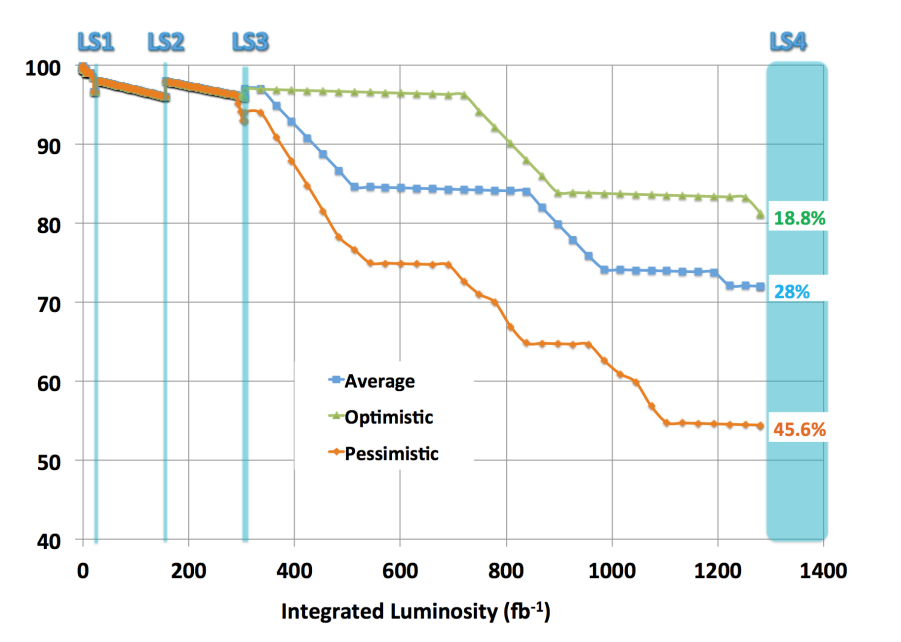
\includegraphics[width=\linewidth]{fig/chapt3/DT-channel-failure.png}
		\caption{\label{fig:DT-failure} Extrapolated fraction of failing channels of the present DT MiC1 electronics as a function of the integrated luminosity for different scenari until LS4~\cite{PHASEIITP}.}
	\end{wrapfigure}

	\acl{DT}s and \acl{CSC}s are important components used to identify and measure muons, especially thanks to their spatial resolution of the order of \SI{100}{\micro m}. Nevertheless, the luminosity and irradiation during HL-LHC will cause serious event loss and ageing on the electronics of these subsystems that will comprise the triggering and data transfering needs of CMS. Thus, electronics upgrade are foreseen to address these expected problems. While only the RPCs' electronic system is able to operate under Phase-2 requirements~\cite{CMSIITP}, DTs and CSCs will need to improve their trigger acceptance rate and latency to ensure that the Level-1 trigger threshold can stay at the same level~\cite{LEVEL1IR}. The Level-1 trigger consists of custom hardware processors receiving data from the calorimeters and the muon system. In return, they generate a trigger signal within \SI{3}{\mu s}, with a maximum rate of \SI{100}{kHz}. In the perspective of HL-LHC, each subsytem needs to achieve a minimum rate of \SI{500}{kHz} with a latency not greater than \SI{12.5}{\micro s}. DTs and CSCs will also need to improve their \acf{DAQ} transfer rate to reach a minimum near \SI{1}{Tbit/s}. The foreseen upgrades are expected to exceed the requirements.
	
\endgroup

\begingroup\setlength{\intextsep}{0pt}\setlength{\columnsep}{15pt}

	\begin{wrapfigure}{l}{.65\linewidth}
		\centering
		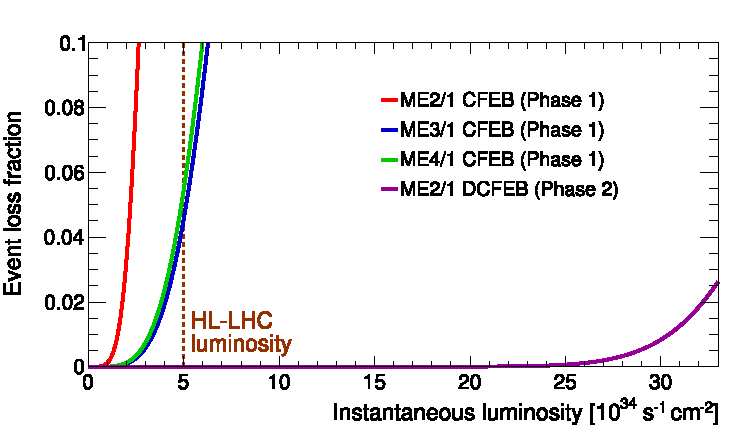
\includegraphics[width=\linewidth]{fig/chapt3/CSC-event-loss.pdf}
		\caption{\label{fig:CSC-event-loss} The event loss fractions as a function of the instantaneous luminosity is compared for CFEBs (Phase-1) and DCFEBs (Phase-2) at different CSC locations. HL-LHC luminosity is marked with the dashed brown line~\cite{PHASEIITP}.}
	\end{wrapfigure}
	
	The \acf{MiC1} used by DTs don't allow for high enough trigger rate. In addition to this problem, it was shown that these electronics contain components that are not radiation hard enough to sustain HL-LHC conditions and hence, a too large number of channels may fail due to radiations as showed in Figure~\ref{fig:DT-failure}. The MiC1 will be replaced on each detector by an improved version referred to as MiC2 while \acf{FEE} and \acf{HV} modules will not need any replacement. On the other hand, CSCs showed that their electronics would be able to live through the 10 years of Phase-2 but the limited buffer depth might cause memory overflows and read-out inefficiencies with a fraction of event loss ranging from 5 to more than 10\% at an instantaneous luminosity similar to which of HL-LHC depending on the expected background. The replacement of CSCs' CFEBs by digital ones, DCFEBs, with deeper buffer would permit to make event loss negligible and satisfy HL-LHC requirements as can be seen in Figure~\ref{fig:CSC-event-loss}. All these new DT and CSC electronics will be connected to the trigger electronics via optical links to ensure a faster communication~\cite{PHASEIITP}.
	
\endgroup

\begingroup\setlength{\intextsep}{0pt}\setlength{\columnsep}{15pt}

	\begin{wrapfigure}{r}{.7\linewidth}
		\centering
		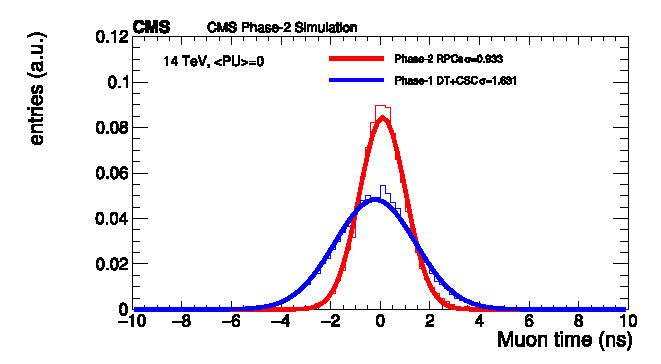
\includegraphics[width=\linewidth]{fig/chapt3/RPC-ugrade-LS.pdf}
		\caption{\label{fig:RPC-time} Comparison of the simulated time residuals in between reconstructed and true muon times without (blue) and with (red) the upgraded RPC link system~\cite{PHASEIITP}.}
	\end{wrapfigure}
	
	The upgrade on the side of Resistive Plate Chambers will not be done at the level of the electronics but rather that of the Link System located in the service cavern of CMS. RPC Link System connects the front-end electronics data of RPCs into CMS trigger processors. The main motivation for such and upgrade is that the electronic board composing the link system are built using obsolete and/or weak components that can easily suffer from the electromagnetic noise. These components may become the source of failing channels throughout Phase-2. Moreover, these link boards were originally designed only to match RPC digitized signals with the corresponding bunch crossing. Due to this feature, the time resolution of the full RPC chain is hence limited to \SI{25}{ns} and does not exploit the full time resolution of the detectors. The time resolution foreseen after the upgrade can be seen through Figure~\ref{fig:RPC-time} and is of the order of \SI{1}{ns}. The exploitation of the full time resolution would make the synchronization of the RPC system easier and allow to have a finer offline out-of-time background removal within the \SI{25}{ns} between consecutive bunch crossings. Moreover, this would greatly improve the trigger and reconstruction on HSCPs. Using the TOF information in between consecutive RPC stations, the minimal particle velocity than could be probed will drop from approximately 0.6 to 0.25 times the speed of light as showed in Figure~\ref{fig:HSCP-trigger}.
	
\endgroup
	
	\begin{figure}[H]
		\begin{subfigure}{0.5\linewidth}
			\centering
			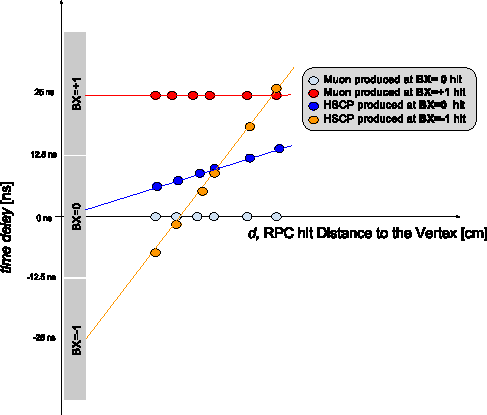
\includegraphics[width = \linewidth]{fig/chapt3/HSCP-RPC-trigger-time.pdf}
			\caption{\label{fig:HSCP-trigger:A}}
		\end{subfigure}
		\begin{subfigure}{0.5\linewidth}
			\centering
			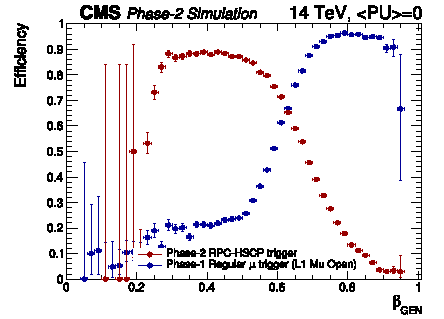
\includegraphics[width = \linewidth]{fig/chapt3/HSCP-RPC-trigger-efficiency.pdf}
			\caption{\label{fig:HSCP-trigger:B}}
		\end{subfigure}
		\caption{\label{fig:HSCP-trigger} Figure~\ref{fig:HSCP-trigger:A}: Time delay with respect to a particle traveling at the speed of light measured at consecutive RPC stations for particles originating at different bunch crossings and traveling at different velocities~\cite{PHASEIITP}. Figure~\ref{fig:HSCP-trigger:B}: In blue is showed the standard level-1 muon trigger efficiency as a function of $\beta$ and in blue is showed the RPC-HSCP trigger efficiency after upgrade of the RPC Link System~\cite{PHASEIITP}.}
	\end{figure}
	
	Upgrading RPC link system will require the installation of 1376 new link boards and 216 control boards. The new boards will make use of the recent progress made with fast FPGAs and will be a great improvement to the ASICs formerly used as they will be able to process signals from several detectors in parallel.

\section{New detectors and increased acceptance}
\label{chapt3:sec:GEMRPC}

	In the present muon system, the redundancy is assured by RPCs used for their robust bunch crossing assignments. The extension of the muon system towards higher pseudo-rapidity in an effort to complete the redundancy and to contribute to the precision of muon momentum measurements will require muon chambers with a spatial resolution less or comparable to the multiple scattering muons are subjected to while traveling through the detector volume~\cite{MUONTDR}. 
	
	\begin{figure}[H]
		\centering
		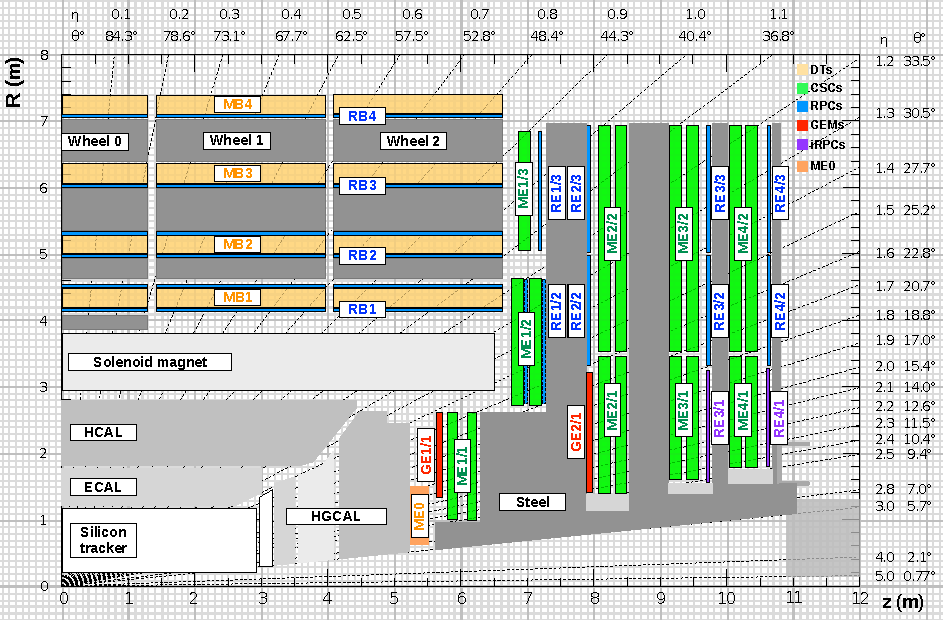
\includegraphics[width=0.9\textwidth]{fig/chapt3/Phase2_Muon_quadrant.pdf}
		\caption{\label{fig:P2Quadrant} A quadrant of the muon system, showing DTs (yellow), RPCs (blue), and CSCs (green). The locations of new forward muon detectors for Phase-2 are contained within the dashed box and indicated in red for GEM stations (ME0, GE1/1, and GE2/1) and dark blue for improved RPC (iRPC) stations (RE3/1 and RE4/1).}
	\end{figure}

\begingroup\setlength{\intextsep}{5pt}\setlength{\columnsep}{15pt}

	\begin{wrapfigure}{r}{.6\linewidth}
		\centering
		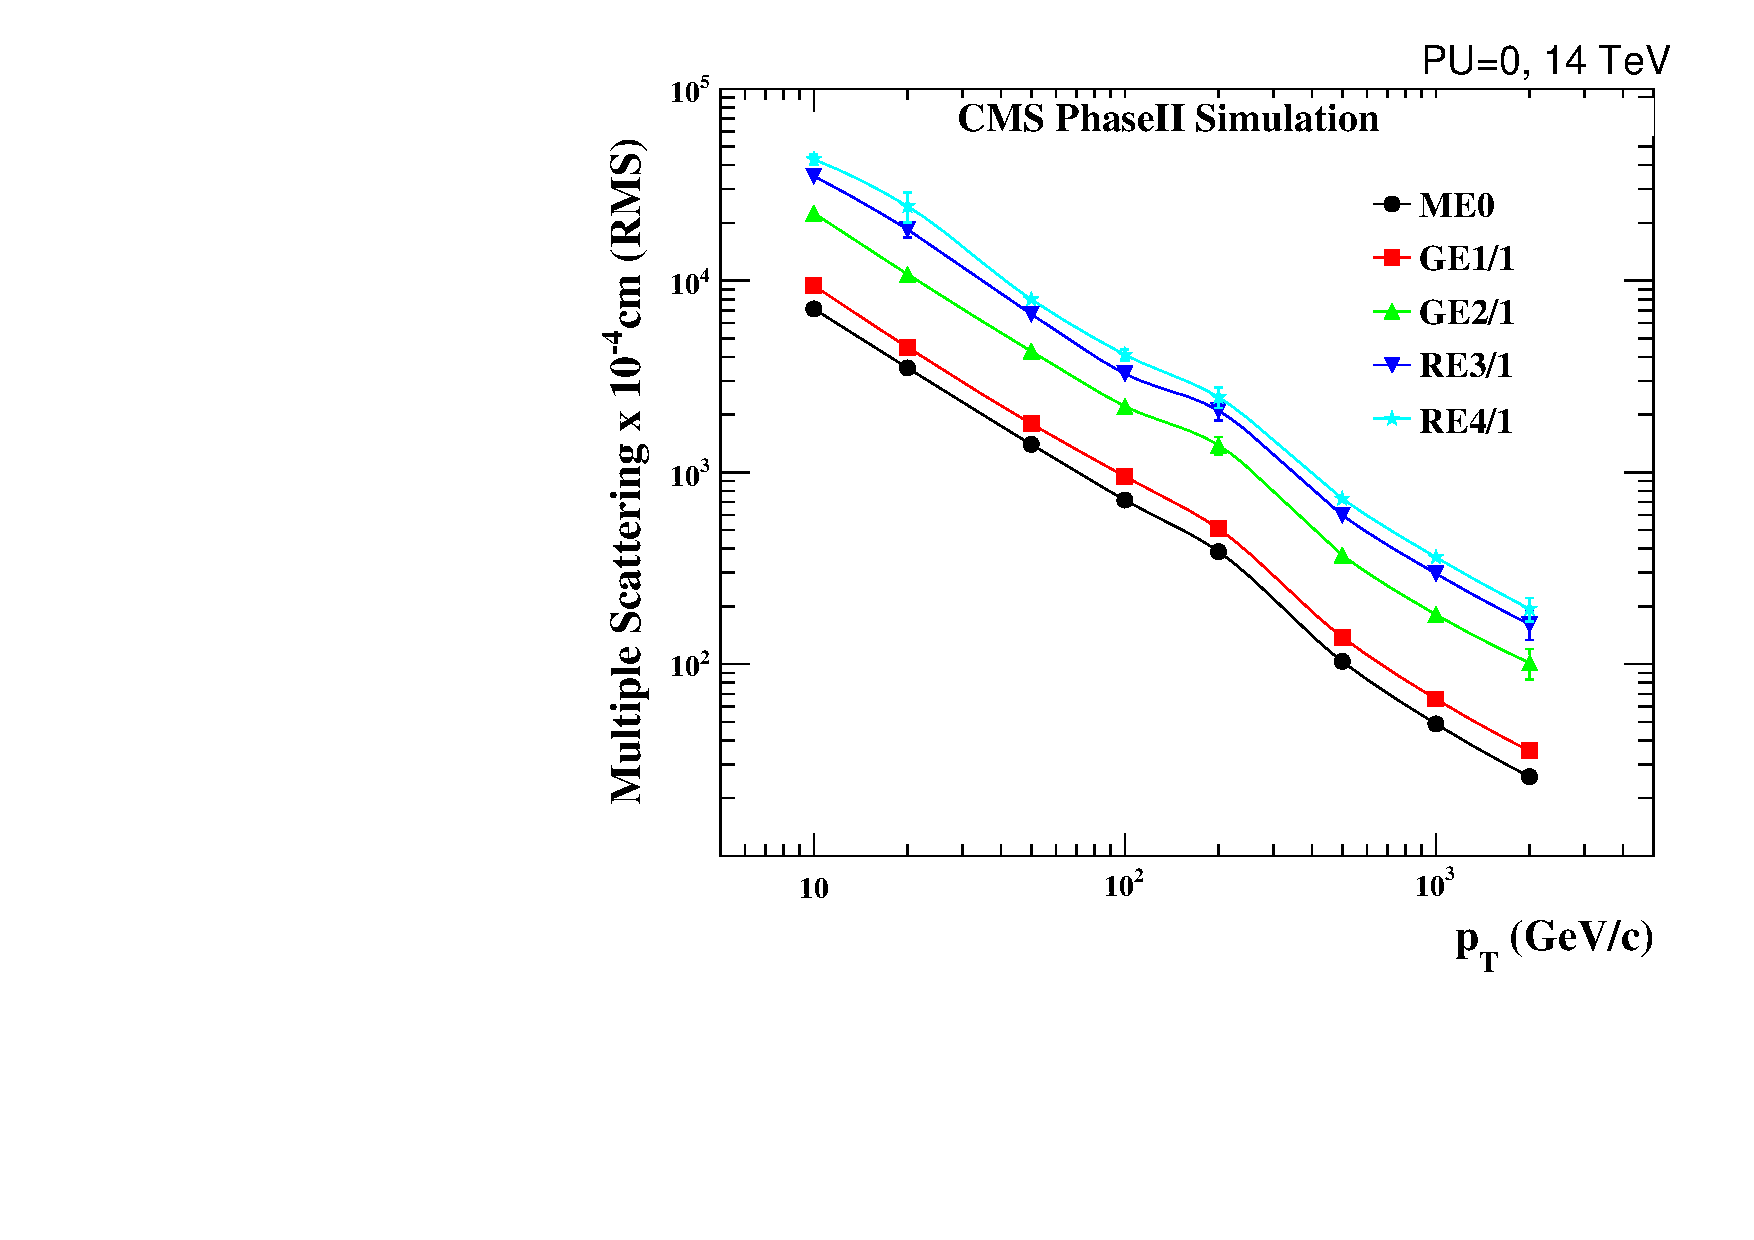
\includegraphics[width=\linewidth]{fig/chapt3/MS_allstations.pdf}
		\caption{\label{fig:MultiScat} RMS of the multiple scattering displacement as a function of muon $p_T$ for the proposed forward muon stations. All of the electromagnetic processes such as bremsstrahlung and magnetic field effect are included in the simulation.}
	\end{wrapfigure}
	
	Figure~\ref{fig:P2Quadrant} shows a similar quadrant of CMS than the one presented in Figure~\ref{fig:Quadrant} with the addition of \acf{GEM} (ME0, GE1/1 and GE2/1) and \acf{iRPC} (RE3/1 and RE4/1) in the pseudo-rapidity region $1.6<\vert\eta\vert<2.4$. The completion of the redundancy was already scheduled in the original CMS Technical Proposal~\cite{CMSTP} but never addressed. The coming Phase-2I is then the occasion to equip the region with the newest GEM and RPC technology. In order to match CMS requirements, a spatial resolution of $\mathcal{O}$(few $\mathrm{mm}$) will be necessary for the proposed new RPC stations while the GEMs will need a resolution better than \SI{1}{mm}, as showed by the simulation in Figure~\ref{fig:MultiScat}. Indeed, most of the plausible physics will be covered only considering muons with $p_T\!\!<$\SI{100}{GeV}.
	
\endgroup
	
	\subsection{Gas electron multipliers}
	\label{chapt3:ssec:GEMs}

\begingroup\setlength{\intextsep}{5pt}\setlength{\columnsep}{15pt}

	\begin{wrapfigure}{r}{.5\linewidth}
		\vspace{-5mm}
		\centering
		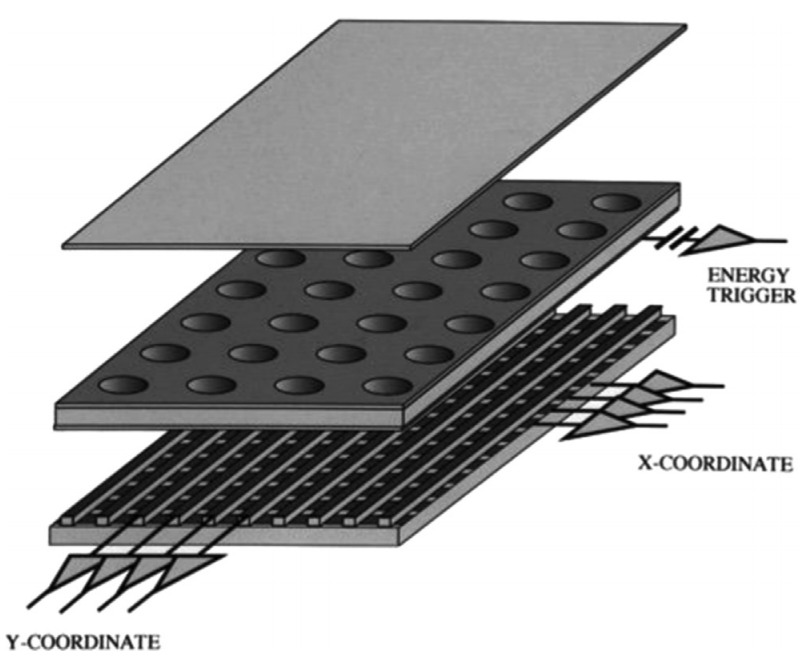
\includegraphics[width=0.9\linewidth]{fig/chapt3/GEM.png}
		\caption{\label{fig:GEM} Schematics of a GEM showing the cathode on top, the GEM foil separating the gas volume into the drift region, in between the cathode and foil, and the induction region, in between the GEM foil and the anode, and finally the anode on which a 2D read-out is installed. A negative voltage is applied on the cathode. The anode is connected to the ground.}
	\end{wrapfigure}
	
	In the region closer to the interaction point where the spatial resolution is requested for the new detectors to be better than \SI{1}{mm} (at least for ME0 and GE1/1 according to Figure~\ref{fig:MultiScat}) and where the background rate will be the highest for muon detectors, the choice has been made to use triple GEMs, micro pattern gaseous detectors, instead of the originally planed RPCs. The GE1/1 project has been the first to be approved and demonstratrators have been installed in CMS already during LS1. The rest of the detectors will be installed during LS2 while the GE2/1 and ME0 projects are still under development. ME0, GE1/1 and GE2/1 will be installed respectively close to the HCAL endcap, on the first and on the second muon endcap disks as can be seen from Figure~\ref{fig:P2Quadrant}.
	
\endgroup

\begingroup\setlength{\intextsep}{5pt}\setlength{\columnsep}{15pt}

	\begin{wrapfigure}{r}{.5\linewidth}
		\centering
		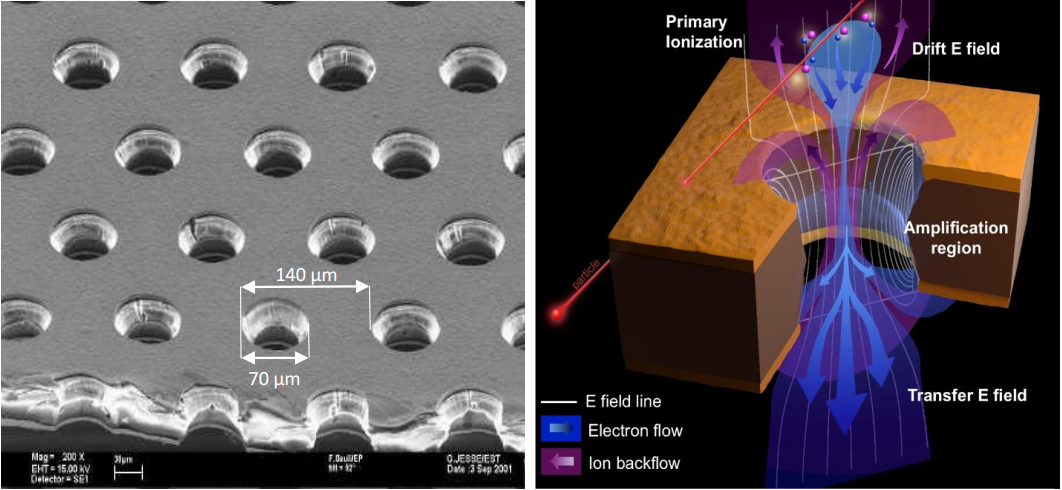
\includegraphics[width=0.7\linewidth]{fig/chapt3/GEM-foil-ampli.png}
		\caption{\label{fig:GEM-foil} Top: Picture of a CMS GEM foil provided by a scanning electron microscope. Bottom: Representation of the electric field in a GEM hole and of the amplification electrons and ions undergo due to the very intense electric field.}
	\end{wrapfigure}
	
	\acl{GEM}s are gaseous detectors~\cite{SAULI97} whose gas volume is confined between two planar electrodes, the anode serving as read-out panel. The gas volume is divided in two or more regions by a single or multiple \textit{GEM foils} as showed in Figure~\ref{fig:GEM}. These foils are very thin, of the order of a few tens of \si{\micro m}, and are pierced with holes as can be seen in Figure~\ref{fig:GEM-foil}. Both surfaces of the GEM foils are clad with copper in order to apply a strong electric field in between each side that will generate very strong potentials in the holes. The gas region contained in between the cathode and the GEM foil is called the drift region as the electric field is not strong enough to cause avalanches and thus start an amplification. The primary electrons drift toward the foil and are accelerated and amplified by the very high potential within the holes, as showed in Figure~\ref{fig:GEM-foil}. Then the electrons reach the second drift region in which they will induce signal on the read-out located on the anode. By restraining the amplification process at the level of the holes, the electrons can stay in a very confined space and thus induce a very localized current, providing the GEMs with a very good spatial resolution.
	
\endgroup

\begingroup\setlength{\intextsep}{5pt}\setlength{\columnsep}{15pt}

	\begin{wrapfigure}{r}{.65\linewidth}
		\vspace{-5mm}
		\centering
		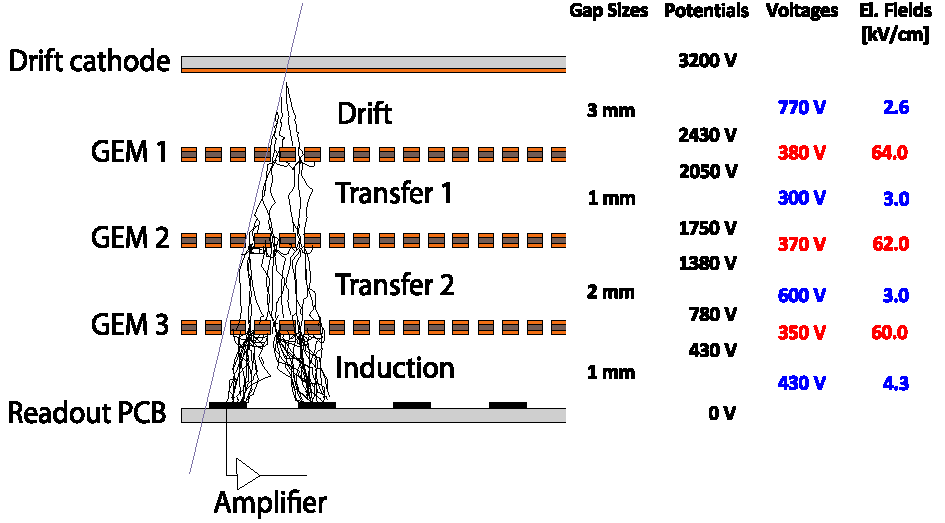
\includegraphics[width=\linewidth]{fig/chapt3/GEM-drift.pdf}
		\caption{\label{fig:GEM-drift} Schematic representation of CMS triple GEMs. The gas volume is divided into four areas. The drift area is the region where the primary electrons are created before being amplified a first time while passing through the first GEM foil. Then the process of drift and amplification is repeated twice in following two transfer areas and GEM foils. Finally, the charges have been amplified enough to induce current in the read-out strips while in the last drift area. The typical dimensions, potentials and electric fields are provided.}
	\end{wrapfigure}
	
	The process can be repeated several times in a row, in order to achieve a stronger amplification. The GEMs that will be used in CMS are triple-GEM detectors operated with a 70/30 gas mixture of $Ar$/$CO_2$. They contain three GEM foils and hence three electron amplifications, as can be seen in Figure~\ref{fig:GEM-drift}. The GEM foils used in CMS are \SI{50}{\micro m} foils clad with \SI{5}{\micro m} of copper on each side. The foils are pierced with double-canonical holes which inner and outer diameters are respectively 50 and \SI{70}{\micro m} which are placed \SI{140}{\micro m} from each other in an hexagonal pattern, as showed in Figure~\ref{fig:GEM-foil}. These detectors have a time resolution better than \SI{10}{ns} and reach very good spatial resolutions of less than \SI{200}{\micro rad} as indeed the position of the hits is not measured along the strips but following the azimuthal angle granularity of the radialy organized trapezoidal strips.
	
\endgroup
	
	The GEM Upgrade project started with GE1/1~\cite{GEM11TDR}. GE1/1 detectors will already be installed during LS2. GE2/1 and ME0, on the other hand, will profit of the R\&D knowledge and skills developed for GE1/1 while the requirements for each subsystem are different as they are not placed at the same distance from the interaction point. In this very forward region, a different position with respect to the center of the detector can change dramatically the conditions in which the detectors will have to be operated. In terms of rate capability, GE2/1, which is the furthest, is required to withstand \SI{2.1}{kHz/cm^2} while GE1/1 needs to be better than \SI{10}{kHz/cm^2} and ME), better than \SI{150}{kHz/cm^2}. In terms of ageing with respect to charge deposition, ME0 needs to be certified to \SI{840}{mC/cm^2}, GE1/1 to \SI{200}{mC/cm^2} and GE2/1 only to \SI{9}{mC/cm^2}. All 3 detectors need to have a time resolution better than \SI{10}{ns} and an angular resolution better than \SI{500}{\micro rad}.
	
	On each GE1/1 ring, 36 super chambers, consisting of two single GEM layers and spanning \SI{10}{\degree}, will be installed covering the pseudo-rapidity region \psrapr{1.6}{2.2} together with ME1/1 CSCs. The reach of the muon system will be improved thanks to the GE2/1 that will overlap with the GE1/1 and cover a region from \psrapg{1.6} to \psrapl{2.4} and complete the redundancy of ME2/1. The super chambers, built with two triple-GEM layers each consisting of four single GEM modules due to the rather large surface of the GE2/1 chambers, that will be installed on the first ring of the second endcap will span \SI{20}{\degree} each. Hence, a total of 72 chambers will be assembled to equip the muon system. Finally, the ME0 installed near the HCAL endcap will cover the region \psrapr{2.0}{2.8}. This subsystem will consist in super modules of six layers of triple-GEM detectors covering an azimuthal angle of \SI{20}{\degree} leading to the construction of 216 single detectors.
	
	Adding the GEMs into the forward region of the muon system will allow to strongly enhance the Level-1 Trigger performance as shown in Figure~\ref{fig:GEM-Trigger}. In the region \psrapr{1.6}{2.4}, the trigger efficiency of the current system would lie between 80 and 90\% under HL-LHC conditions. The installation of GEMs would bring the efficiency to a consistent 92 to 94\% on the entire region. At the same time, the trigger rate is expected to fluctuate from 3 to \SI{10}{kHz} with the current system alone. The addition of detectors to complete the redundancy would allow to keep the rate mostly under \SI{2}{kHz}. Moreover, benefiting from the good spatial and angular resolution of the GEMs, the precision into the muon measurement will also be improved by an order of magnitude thanks to the addition of GEMs as can be seen from the simulation presented in Figure~\ref{fig:GEM-Muon}. 

	\begin{figure}[H]
		\begin{subfigure}{0.5\linewidth}
			\centering
			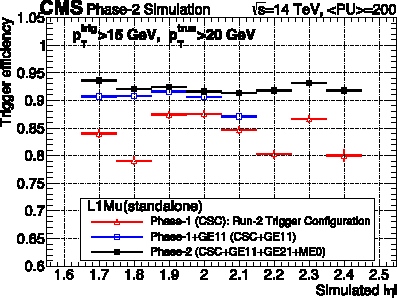
\includegraphics[width=.9\linewidth]{fig/chapt3/GEM-Trigger-efficiency.pdf}
			\caption{\label{fig:GEM-Muon:A}}
		\end{subfigure}
		\begin{subfigure}{0.5\linewidth}
			\centering
			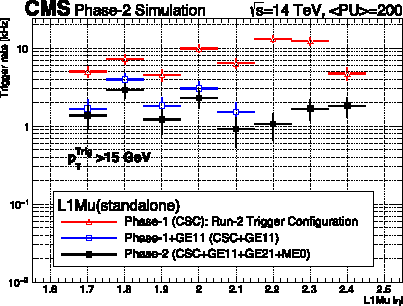
\includegraphics[width=.9\linewidth]{fig/chapt3/GEM-Trigger-rate.pdf}
			\caption{\label{fig:GEM-Muon:B}}
		\end{subfigure}
		
		\caption{\label{fig:GEM-Trigger} Simulated efficiency and rate of the standalone Level-1 muon trigger using tracks reconstructed in CSCs and all GEM stations compared with Phase-1 values in the case where only CSCs are used or CSCs+GE1/1. The zones of inefficiency of the CSC subsystem are compensated by the addition of GEMs during Phase-2 and the trigger rates is kept from increasing due to the high luminosity~\cite{PHASEIITP}.}
	\end{figure}
	
	\begin{figure}[H]
		\begin{subfigure}{0.5\linewidth}
			\centering
			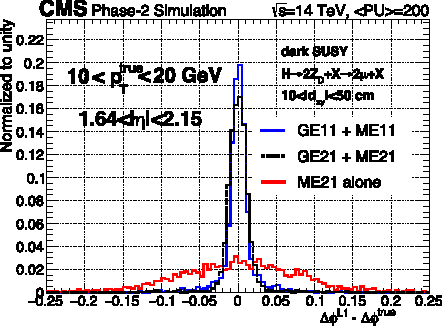
\includegraphics[width=.9\linewidth]{fig/chapt3/GEM-muon-direction.pdf}
			\caption{\label{fig:GEM-Muon:A}}
		\end{subfigure}
		\begin{subfigure}{0.5\linewidth}
			\centering
			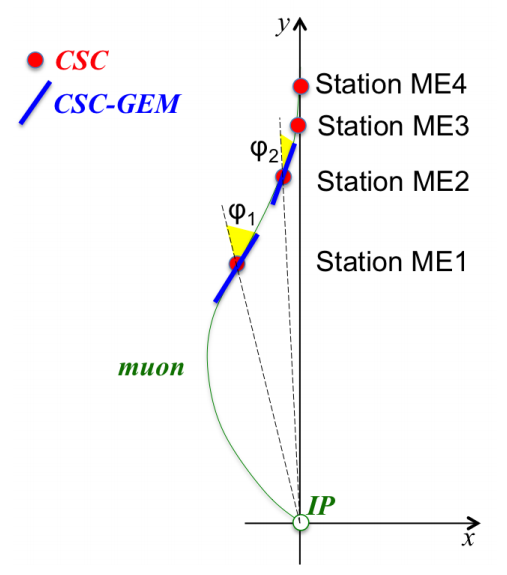
\includegraphics[height=5cm]{fig/chapt3/GEM-muon-bending.png}
			\caption{\label{fig:GEM-Muon:B}}
		\end{subfigure}
		\caption{\label{fig:GEM-Muon} Figure~\ref{fig:GEM-Muon:A}: Simulated resolution of the muon direction measurement $\Delta\phi$ with Phase-2 conditions. In the second endcap station, the resolution is compared in the case of CSCs (ME2/1) alone and CSCs+GEMs (GE2/1+ME2/1) while a similar resolution measurement is given in the case of the first station (GE1/1+ME1/1)~\cite{PHASEIITP}. Figure~\ref{fig:GEM-Muon:B}: The addition of GEM detectors on stations 1 and 2 (ME0 is considered to contribute to station station 1) as redundant system to CSCs allows to improve the muon momentum improvement through a more accurate measurement of the local bending angles $\phi_1$ and $\phi_2$~\cite{PHASEIITP}.}
	\end{figure}
	
	\subsection{Improved forward resistive plate chambers}
	\label{chapt3:ssec:iRPCs}
	
	Figure~\ref{fig:P2Quadrant} shows that the iRPCs that will equip the third and fourth endcap disks in position RE3/1 and RE4/1 will finally be the partners of the CSCs in position ME3/1 and ME4/1. They will complete Phase-1 plans by bringing the needed upgrades in the perspective of Phase-2 as the older chambers are not suitable to equip the forward region of CMS due to HL-LHC rates and charge deposition. By completing the redundancy, more hits along the muon track will be available and the lever arm will be improved. The benefits from extending the redundancy of the muon system with iRPCs to the forward most region is shown in Figure~\ref{fig:Endcap-trigger-eff} in which the trigger efficiency is presented with and without RPCs. It is possible to see that the efficiency of the CMS muon trigger with the complete redundancy is consistently improved to a level above 95\% in the region \psrapg{1.8} as the iRPCs help filling the holes in the CSC system.

	\begin{figure}[H]
		\begin{subfigure}{0.5\linewidth}
			\centering
			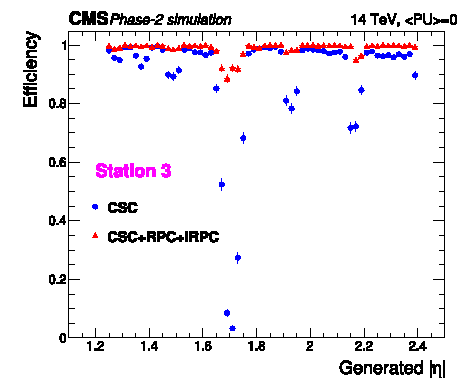
\includegraphics[width=\linewidth]{fig/chapt3/Trigger-efficiency-endcap-3.pdf}
			\caption{\label{fig:Endcap-trigger-eff:A}}
		\end{subfigure}
		\begin{subfigure}{0.5\linewidth}
			\centering
			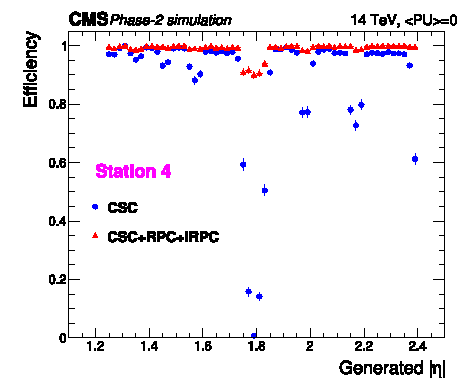
\includegraphics[width=\linewidth]{fig/chapt3/Trigger-efficiency-endcap-4.pdf}
			\caption{\label{fig:Endcap-trigger-eff:B}}
		\end{subfigure}
		\caption{\label{fig:Endcap-trigger-eff} Simulation of the impact of RPC hit inclusion onto the local trigger primitive efficiency in station 3 (Figure~\ref{fig:Endcap-trigger-eff:A}) and station 4 (Figure~\ref{fig:Endcap-trigger-eff:B})~\cite{PHASEIITP}. The contribution of iRPC starts above \psrape{1.8}.}
	\end{figure}
	
	The detectors that will be installed in the coming years will have similarities with the already existing RPC system. 18 of the new chambers, each spanning \SI{20}{\degree} in $\varphi$ around the beam axis with 96 radially oriented trapezoidal read-out strips, will cover each muon endcap disk leading to the production of 72 iRPCs. The main difference with the old RPC detectors will be found at the level of the read-out panels. Indeed, the new chambers will not feature read-out strips segmented in $\eta$ but rather will favor a read-out on both strip ends to determine the position of the hits along the chamber. By using fast front-end electronics a radial spatial resolution of the order of \SI{2}{cm} could be achieved to contribute to the better reconstruction of muons in the forward region where the bending due to the magnetic field is low. This technical choice is motivated by the fact that, in the case a $\eta$ segmentation were to be used used, at least five pseudo-rapidity partitions would have been necessary to reach the minimal radial spatial resolution ($\approx$ \SI{20}{cm}). Having only one strip along the chamber read-out from both ends reduces by 60\% the total number of channels and the necessary cabling, and allows for a better spatial resolution. The strip pitch will range from \SI{6.0}{mm} (\SI{5.9}{mm}) on the high pseudo-rapidity end to \SI{12.3}{mm} (\SI{10.9}{mm}) on the low one on position RE3/1 (RE4/1). The spatial resolution in the direction perpendicular to the strips should reach approximately \SI{3}{mm}, better than the minimal needed resolution (Figure~\ref{fig:MultiScat}). Finally, the overall time resolution of the new installation will be equally \SI{1}{ns}, as for the present due to the same link system being used even though the detector itself can achieve a time resolution of less than \SI{100}{ps}, necessary for a spatial reconstruction of the hits with a resolution of \SI{2}{cm} or less along the strip length.
	
	Having only a single strip instead of pseudo-rapidity segmentation will increase the probability of double hits in the same channel. The probability was estimated to be low enough as it shouldn't exceed 0.7\%. This estimation was made assuming an average hit rate per unit area of \SIrate{600} in the iRPCs (see Figure~\ref{fig:iRPC-Rate}), a cluster size (average number of strips fired per muon) of 2, a strip active area of \SIsurface{158.4}{0.87}{cm} and a safety factor 3. The corresponding rate per strip is estimated to be \SI{380}{kHz} leading to an average time interval in between two consecutive hits of \SI{2600}{ns}. This is compared to the minimal time interval of \SI{16}{ns} necessary to avoid ambiguities. Indeed, a maximum of \SI{10}{ns} is spent by the signal traveling through the strip to reach the electronics to which can be added \SI{1}{ns} of dead time and 2 \acf{TDC} clock cycles of \SI{2.5}{ns} to convert the signal arrival time into a digital value in the FEEs. The probability of having ambiguous double hits in a strip is then the ratio between the minimal time interval in between two consecutive hits and the average time interval estimated from the rate the detectors would be subjected to.

	\begin{figure}[H]
		\centering
		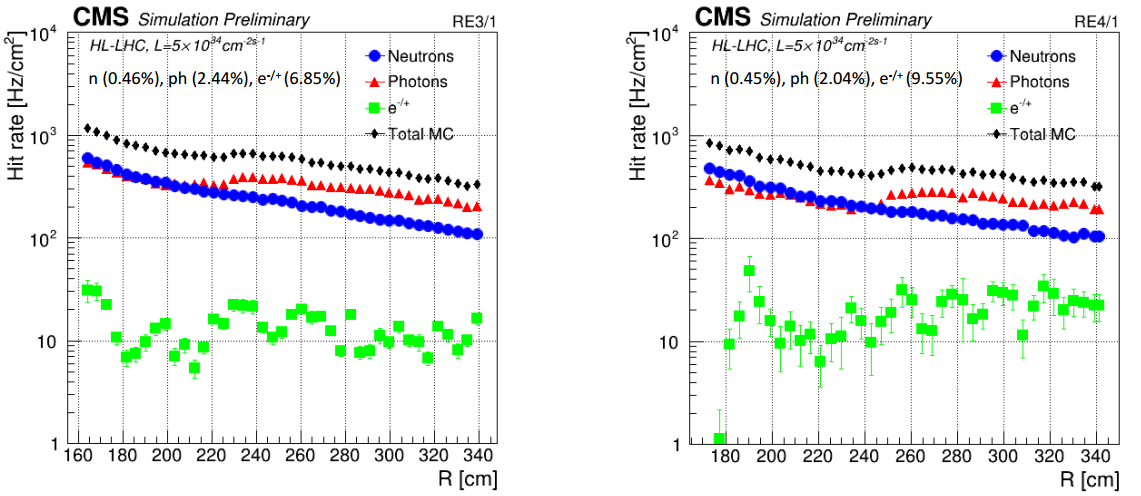
\includegraphics[width=\textwidth]{fig/chapt3/RPC-Sim-HL-LHC_Rate.png}
		\caption{\label{fig:iRPC-Rate} Expected hit rate due to neutrons, photons, electrons and positrons at HL-HLC instantaneous luminosity of $5\times10^{34}$ \si{cm^{-2}s^{-1}} in RE3/1 and RE4/1 chambers~\cite{ANDREA2018,ANDREA2018PROC}. The sensitivities of iRPCs used in the simulation for each particle are reported and differ from one endcap disk to another as the energies of the considered particles varies with the increasing distance from the interaction point.}
	\end{figure}
	
	The instantaneous luminosity at HL-LHC being very high, the rates at the position of the new chambers needed to be simulated in order to understand the necessary requirements for these detectors. The simulated results for different background components (neutrons, photons, electrons and positrons) are shown in Figure~\ref{fig:iRPC-Rate} assuming known sensitivities to these particles. It is shown that on average over the iRPC areas the rates would be of the order of \SIrate{600} (\SIrate{600} seen in RE3/1 and \SIrate{480} in RE4/1)~\cite{ANDREA2018,ANDREA2018PROC}. Thus, taking into account a safety factor of about 3, it was decided that improved RPCs should at least be certified for rates reaching \SIrate{2} which will be achieved thanks to several improvements on the design and on the electronics. The detectors design will be based on the existing RPCs as they will also feature double RPC gaps. Similarly to the existing RPC system, the electrode material will be HPL although the thickness of the electrodes and of the gas gap will be reduced to \SI{1.4}{mm} as a thinner gas gap leads to a decrease of deposited charge per avalanche as showed in Figure~\ref{fig:charge-gap}. The charge deposition in the case of \SI{1.4}{mm} thick electrodes is reduced by a factor greater than 5 when compared to \SI{2}{mm} electrodes at similar electric field. The smaller the gas gap, the more the detector becomes sensitive to gap non-uniformities across the electrode planes, making a gap of \SI{1.4}{mm} a good compromise in between these two competing factors.

\begingroup\setlength{\intextsep}{5pt}\setlength{\columnsep}{15pt}

	\begin{wrapfigure}{r}{.55\linewidth}
		\centering
		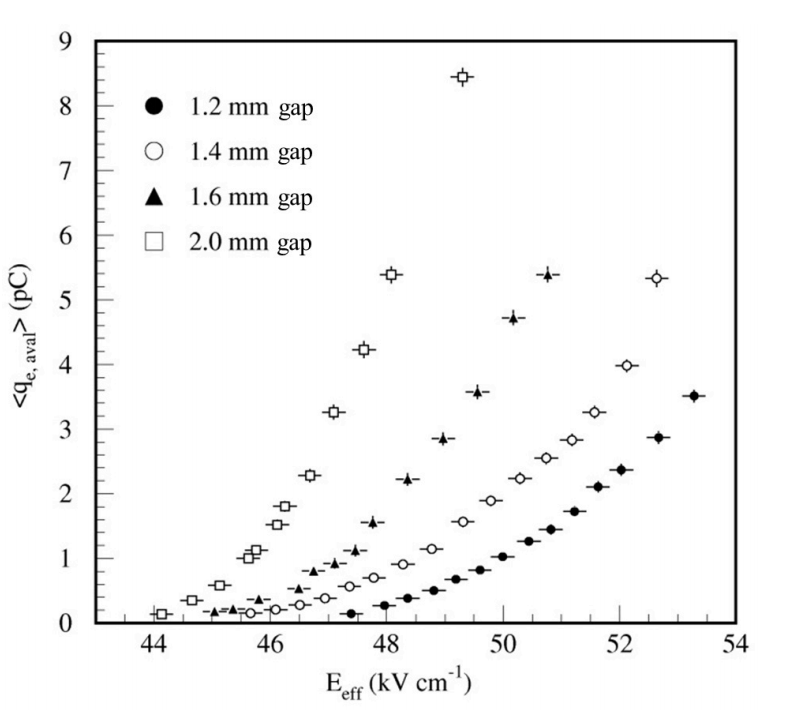
\includegraphics[width=\linewidth]{fig/chapt3/charge-vs-gap.png}
		\caption{\label{fig:charge-gap} Measured average charge per avalanche as a function of the effective electric field for different gas gap thickness in double-gap RPCs using HPL electrodes~\cite{PHASEIITP}.}
	\end{wrapfigure}
	
	A lower charge deposition inside of the detector volume means a slower ageing and a longer lifetime for detectors subjected to high irradiation. But, in order to take advantage of the lower detector gain, more sensitive electronics are required such that part of the gain that was formerly achieved in the gas volume can be moved to the electronics. Achieving this with the technology developed more than ten years ago for the present system is not possible as the signal over noise ratio of such electronics doesn't allow to detect charges as low as \SI{10}{fC}. Moreover, the new front-end electronics will need to be radiation hard to survive more than ten years of HL-LHC conditions. The new technology that has been chosen is based on the PETIROC ASIC manufactured by OMEGA and is a 64-channel ASIC called CMS RPCROC\cite{PETIROCIEEE,PETIROCTWEPP,PHASEIITP}. The properties of these electronics will be discussed in Chapter~\ref{chapt6}.
	
\endgroup
	
%	\subsection{Installation schedule}
%	\label{chapt3:ssec:schedule}
%	
%	The previous discussion on the different upgrade projects makes it clear that a lot of work is schedule for CMS to be ready at the end of LS3 for HL-LHC. Conducting all the upgrades of the muon system together with upgrades of the other subsystems like the replacement of the Tracker and of part of the ECAL, will prove to be very difficult as the opening of CMS to access the Barrel will be done by fully opening the endcaps leaving only the first disk to be accessible. Thus, most subsystems have planed early installation over LS2, and the following YETS until LS3 in order to give more space to LS3 schedule.
%	
%	First of all, LS2 will see the installation of GE1/1 detectors, all the on-detector schedule of CSCs and the installation of the necessary services for the improved RPCs to be installed later, such as the HV and LV power supply lines, the gas and cooling lines or signal cables. CSCs will have a huge work to do during LS2 as they will need to extract all of their detectors to refurbish them with upgraded DCFEB and ALCT mezzanine boards. The GE1/1 services were installed during LS1 together with a few demonstrator and only the detectors needs to be integrated into the first endcap disk. The detectors are presently being built and tested at the different assembly site to prepare for a smooth LS2 work.
%	
%	The work of GEMs will be continued during the following YETS during which is planned the installation of the GE2/1 stations to only leave the ME0 to be installed during LS3. The iRPC program will follow a similar path as the new detectors will be installed during the YETS preceding LS3 in prevision of the fact that the endcap disks will not be accessible during LS3. This way, all the subsystems, but DTs, made great effort on planing their installation and integration within CMS only to have to deal with off-detector issues during the LS3 period, such as the replacement of ODMBs and HV system in the case of CSCs or the upgrade of the RPC Link System. Finallly, during LS3 are schedules the replacement of DT minicrates electronics and the installation and integration of ME0 GEMs together with the HGCAL.
	
\section{Impact on Level-1 Trigger and physics performance}
\label{chapt3:sec:L1tP2}

\begingroup\setlength{\intextsep}{5pt}\setlength{\columnsep}{15pt}

	\begin{wrapfigure}{l}{.5\linewidth}
		\centering
		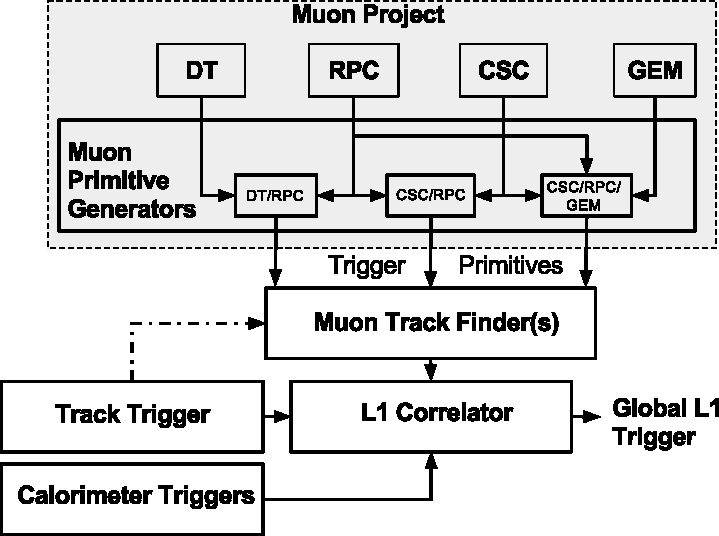
\includegraphics[width=\linewidth]{fig/chapt3/Phase-II-L1-Trigger.pdf}
		\caption{\label{fig:L1-trigger} Level-1 Trigger data flow during Phase-2 operations~\cite{PHASEIITP}.}
	\end{wrapfigure}

	The upgrades of the different subsystems will have a subsequent impact on the Level-1 Trigger. Indeed, although its main scheme will not be affected, the efficiency of the trigger in identifying muons and provide the DAQ with good and fast trigger that can cope with HL-LHC instantaneous luminosity is a major improvement. In addition to the upgrade of the muon system in terms of trigger accept rate and latency, the Level-1 Trigger will get extra information by including the Tracker Trigger into its Muon Track Finder logic and combine the L1 Muon Trigger with Tracker and Calorimeter Triggers to generate a Global L1 Trigger, as shown in Figure~\ref{fig:L1-trigger}. Using the track candidates of both the muon system and the tracker in spatial coincidence will allow for a much better momentum resolution thanks to better identified muons and, hence, better measured transverse impulsion as described in reference~\cite{PHASEIITP}.
	
\endgroup
	
	In terms of muon trigger, three regions are considered due to their different track finding logic: the \acf{BMTF}, the \acf{EMTF} for both the barrel and endcap regions, and finally the \acf{OMTF} which concerns the pseudo-rapidity region in which there is a common coverage by both the barrel and endcap muon systems. This region can be seen in Figure~\ref{fig:P2Quadrant} for \psrapr{0.9}{1.2} and requires a specific more complex logic to provide an efficient reconstruction of muons due to the different orientation of the detectors and of the more complex magnetic field of this region. The development of a track finder specific to the overlap region was achieved during the Phase-1 upgrade of the L1-Trigger~\cite{L1UPGRADE2016}.
	
	The upgraded RPC link system, allowing to take profit of the full \SI{1}{ns} resolution of the detectors, will help reducing the neutron induced background, slightly improve the bunch crossing assignment, and help increasing the trigger efficiency in every sector. The upgrade of DT electronics is also to take into account as the trigger primitive generator will be renewed through the use of TDCs that will send the digitized signals directly to common DT/RPC back-end electronics instead of having an on-detector trigger logic as it will be the case until the end of Phase-1. The combination of RPC hits together with DT primitives will bring extra improvement in the bunch crossing assignment in the barrel and overlap regions and improve the efficiency of the trigger between the wheels were the quality of DT primitives is the poorest.

	\begin{figure}[H]
		\begin{subfigure}{0.5\linewidth}
			\centering
			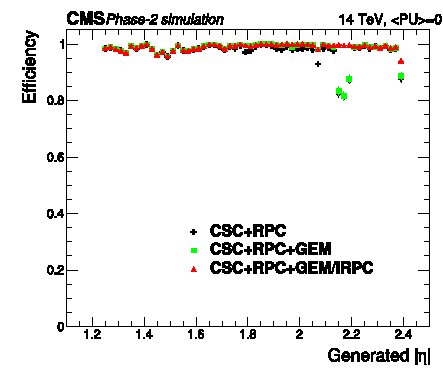
\includegraphics[width=\linewidth]{fig/chapt3/EMTF-eff-2of4.pdf}
			\caption{\label{fig:EMTF-eff:A}}
		\end{subfigure}
		\begin{subfigure}{0.5\linewidth}
			\centering
			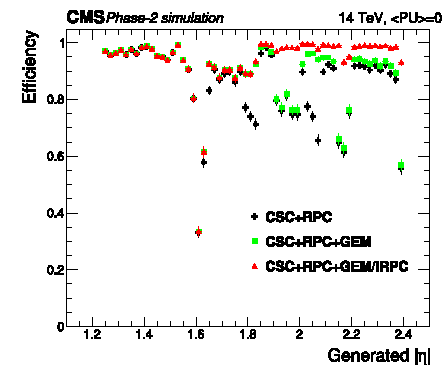
\includegraphics[width=\linewidth]{fig/chapt3/EMTF-eff-4of4.pdf}
			\caption{\label{fig:EMTF-eff:B}}
		\end{subfigure}
		\caption{\label{fig:EMTF-eff} Efficiency of the L1 trigger in the endcap region after Phase-2 upgrade in the case CSC/GEM/RPC hits are requested in at least 2 stations out of four (\ref{fig:EMTF-eff:A}) and in all four stations (\ref{fig:EMTF-eff:B})~\cite{PHASEIITP}.}
	\end{figure}

	The current EMTF already uses more sophisticated algorithms by combining together RPC hits and CSC primitives. The GEMs, in stations 1 and 2, and the iRPCs, in stations 3 and 4, will be added into the EMTF algorithm. Both these contributions will help increasing the efficiency of the L1 trigger in the endcap region in one hand, as showed by Figure~\ref{fig:EMTF-eff}, and help lowering the L1 trigger rate in the other hand, especially in the most forward region. Similarly to the RPC/CSC algorithms, data from both CSCs and GEMs are combined into the \acf{OTMBs} to build on each station, GEM/CSC primitives matching space and time information from both subsystems. The efficiency improvement and rate reduction close to the beam line will be naturally enhanced by the addition of more hits along the muon tracks, as can be seen from Figure~\ref{fig:CSC-GEM-perf} that focuses especially in the most challenging pseudo-rapidity region. Indeed, the contribution from the GEMs to the lever arm of each track thanks to their high angular resolution will be a great asset in achieving such results, as can be seen in Figure~\ref{fig:CSC-GEM-res}. The rate will be partly reduced in the forward region thanks to the better spatial resolution of iRPCs, with respect to the current RPC system. The ambiguity brought by multiple local charged tracks in CSCs will be reduced, as explained through Figure~\ref{fig:LCT-ambiguity}. Indeed, as the rates will increase, the probability to record more than a single local charged track will greatly increase. This is due to the fact that the trigger algorithm uses information from three consecutive bunch crossings to find muon tracks. It is estimated that with iRPCs operated at 95\% efficiency the resolution of ambiguous events would be of the order of 99.7\%.
	
	\begin{figure}[H]
		\begin{subfigure}{0.5\linewidth}
			\centering
			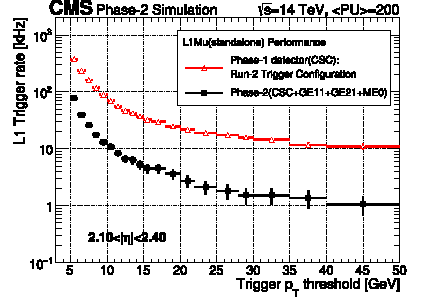
\includegraphics[height=5cm]{fig/chapt3/GEM-trigger-rate.pdf}
			\caption{\label{fig:CSC-GEM-perf:A}}
		\end{subfigure}
		\begin{subfigure}{0.5\linewidth}
			\centering
			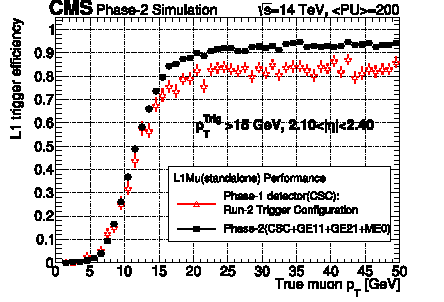
\includegraphics[height=5cm]{fig/chapt3/GEM-trigger-eff.pdf}
			\caption{\label{fig:CSC-GEM-perf:B}}
		\end{subfigure}
		\caption{\label{fig:CSC-GEM-perf} Comparison of L1 trigger performances for prompt muons with and without the addition of GEMs in the region \psrapr{2.1}{2.4} at Phase-2 conditions~\cite{PHASEIITP}. GEMs would allow a reduction of the trigger accept rate by an order of magnitude (Figure~\ref{fig:CSC-GEM-perf:A}) while increasing the trigger efficiency (Figure~\ref{fig:CSC-GEM-perf:B}).}
	\end{figure}
	
	\begin{figure}[H]
		\begin{subfigure}{0.5\linewidth}
			\centering
			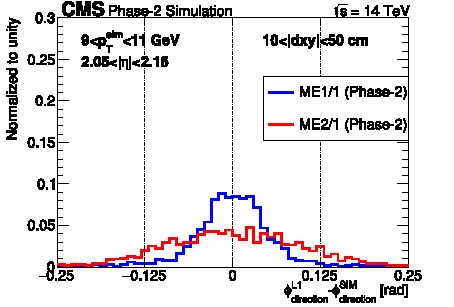
\includegraphics[height=5cm]{fig/chapt3/CSC-angular-res.pdf}
			\caption{\label{fig:CSC-GEM-res:A}}
		\end{subfigure}
		\begin{subfigure}{0.5\linewidth}
			\centering
			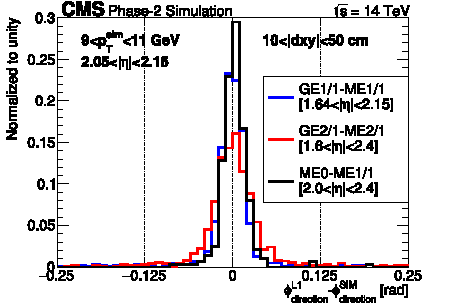
\includegraphics[height=5cm]{fig/chapt3/GEM-angular-res.pdf}
			\caption{\label{fig:CSC-GEM-res:B}}
		\end{subfigure}
		\caption{\label{fig:CSC-GEM-res} The angular resolution on reconstructed muon tracks in the GEM overlap region \psrapr{2.0}{2.15} is compared for Phase-2 conditions in the case CSC are alone (Figure~\ref{fig:CSC-GEM-res:A}) and in the case the GEMs' data, including ME0, is combined to which of CSCs (Figure~\ref{fig:CSC-GEM-res:B})~\cite{PHASEIITP}.}
	\end{figure}

	\begin{figure}[H]
		\centering
		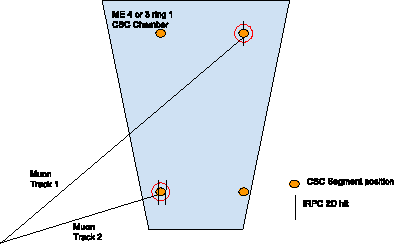
\includegraphics[width=.8\linewidth]{fig/chapt3/CSC-LCT-ambiguity.pdf}
		\caption{\label{fig:LCT-ambiguity} Resolution of the LCT ambiguous events thanks to the combination of CSC and iRPC readout data. Using CSCs only, 2 pairs of hits are possible~\cite{PHASEIITP}.}
	\end{figure}

\section{Ecofriendly gas studies}
\label{chapt3:sec:EcoGas}

	The European Commission adopted a new "F-gas regulation" in 2014~\cite{EUFGAS2014} with the goal to strongly control and reduce the use of fluorinated gases with high \acf{GWP}. Using $CF_4$, $C_2H_2F_4$ and $SF_6$, both CSC and RPC subsystems will need to address this problem by finding new gas mixture for the operation of their detectors. Finding a replacement for these gas component that were used for very specific reasons is a great challenge. Indeed, CSCs use $CF_4$ in order to enhance the longevity of the detectors, increase the drift velocity of electrons and quench photons with a non-flammable gas mixture. RPCs use a mixture mainly composed of $C_2H_2F_4$, or \textit{R134a}, that features a high effective Townsend coefficient and the great average fast charge allowing for operations with a high threshold. The mixure also contains a small fraction of $SF_6$ that is used for its electronegative properties that prevents the development of delta-rays in the gas volume that might trigger multiple ionization and avalanches.
	
	\begin{table}[H]
		\centering
		\begin{tabular}{l c c}
			\hline
			 & CSC & RPC\\
			\hline
			Greenhouse gases used & $CF_4$ & $C_2H_2F_4$ and $SF_6$ \\
			Greenhouse gases fraction in the gas mixture & 10\% & 95.2\% and 0.3\% \\
			Global Warming Potential (relative to $CO_2$) & 6500 & 1300 and 23900 \\
			Gas mixture re-circulation & Yes, 90\% & Yes, 85\% \\
			Gas mixture replenishing rate (\si{l/hr}) & 700 & 1100 \\
			F-gas recuperation & Yes, $\approx$40\% & No \\
			F-gas venting rate (\si{l/hr}) & 42 & 1047 and 3.3 \\
			$CO_2$-equivalent rate (\si{m^3/h}) & 273 & 1440 \\
			Relative impact (entire muon system = 100\%) & 16\% & 84\% \\
			\hline
		\end{tabular}
		\caption{\label{tab:F-GAS-CMS} Details of the greenhouse fluorinated gases used in CMS and of their GWP~\cite{PHASEIITP}.}
	\end{table}
	
	Nevertheless, all these gases have a very high GWP, as reported in Table~\ref{tab:F-GAS-CMS}, and only few options are left. The subsystems need to work on strongly decreasing the loss of these gases due to leaks in the gas system or need to completely change their gas mixture for more ecofriendly ones. Reducing the amount of F-gas released in the atmosphere due to leaks on the current gas system will require installation of a F-gas recuperation system on RPCs side and an upgrade of CSCs existing one in addition to the repair of existing leaks. With such measures, it is expected that the total rate of greenhouses gas vented in the atmosphere would represent only 1.6\% of the current levels~\cite{PHASEIITP}. In the most critical case the F-gas were to be banned, it would be necessary to have replacement mixtures to operate CMS. CSC is presently investigating replacement for $CF_4$ such as $CF_3I$, $C_4F_6$, $IC_3F_6$, $C_3F_8$ or $CHF_3$. RPCs, in collaboration with the ATLAS RPC group which uses the same gas mixture, have identified $CF_3I$ (\GWPleq{1}) and $C_3H_2F_4$ (\GWPsim{6}), referred to as \textit{HFO-1234ze}, as potential candidates with mixtures containing $CO_2$. More R\&D needs to be conducted for both subsystems before concluding on the best alternative. Finding no good alternative to the present mixtures will require very efficient abatement system in CMS to burn and convert the greenhouse gases into less harmful ones. This way, the air pollution would be strongly reduced.
	
	The status of RPC studies are presented in Figure~\ref{fig:RPC-eco} in which the performance (efficiency and streamer probability) of an RPC operated with alternative gas mixtures is compared to the present CMS RPC mixture. Although the efficiency of detectors operated with mixtures containing $CO_2$/$CF_3I$ or $CO_2$/$HFO$ as a replacement for $C_2H_2F_4$ seems to reach similar levels than which of the detectors operated with the present mixture, the new gas mixtures feature a streamer probability (probability to have very large avalanches whose induced charge is greater than \SI{20}{pC}) that far exceeds which of the present fluorinated mixture. The $SF_6$ doesn't seem to prevent the formation of streamers as efficiently even when used at levels more than three times higher than with the standard CMS RPC mixture. Nevertheless, it is important to note that these results were obtained with a single gap RPC while the use of a double gap RPC reduces the operation voltage by 200 to \SI{300}{V}, lowering the induced charge. A compromise in between good efficiency and acceptable level of streamer probability, and the fine tuned composition of potential replacement gas mixtures will be keep on being studied using a standard double-gap CMS RPC.
	
	\begin{figure}[H]
		\hspace*{-0.1\linewidth}
		\begin{subfigure}{0.6\linewidth}
			\centering
			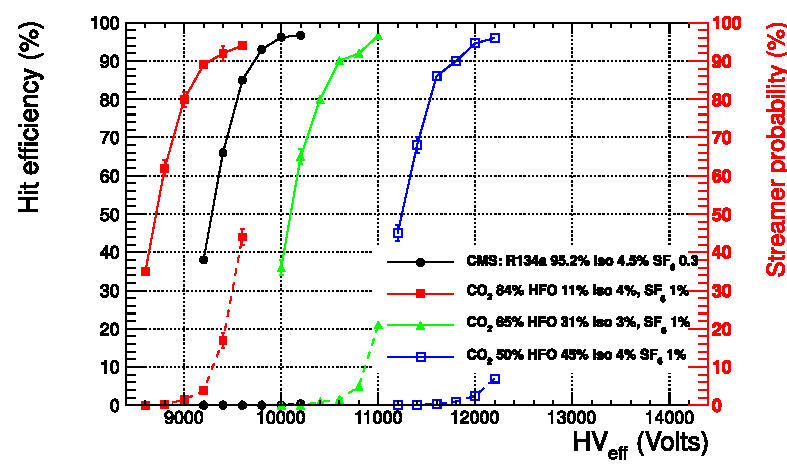
\includegraphics[height=5cm]{fig/chapt3/HFO-mixture.pdf}
			\caption{\label{fig:RPC-eco:A}}
		\end{subfigure}
		\begin{subfigure}{0.6\linewidth}
			\centering
			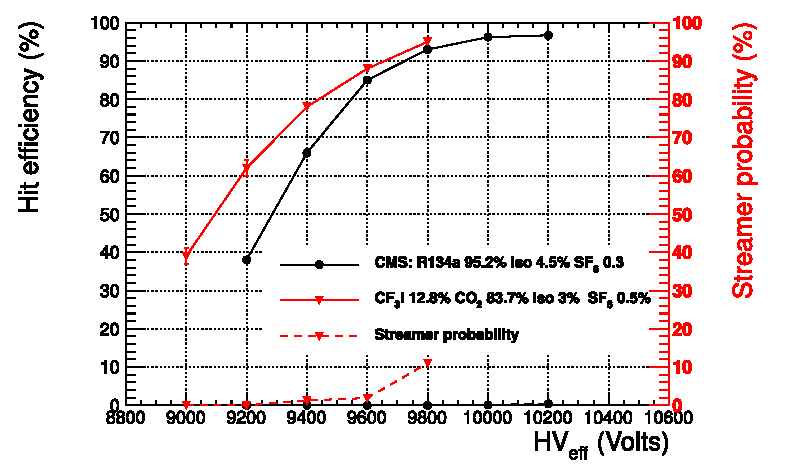
\includegraphics[height=5cm]{fig/chapt3/CF3I-mixture.pdf}
			\caption{\label{fig:RPC-eco:B}}
		\end{subfigure}
		\caption{\label{fig:RPC-eco} The efficiency (solid lines) and streamer probability (dashed lines) of $HFO$/$CO_2$ (Figure~\ref{fig:RPC-eco:A}) and $CF_3I$/$CO_2$ (Figure~\ref{fig:RPC-eco:B}) based gas mixtures as a function of the effective high-voltage are compared with the present CMS RPC gas mixture represented in black~\cite{PHASEIITP}. The detector used for the study is a single gap RPC with similar properties than CMS RPCs. The streamer probability is defined as the proportion of events with a deposited charge greater than \SI{20}{pC}.}
	\end{figure}

\begingroup\setlength{\intextsep}{0pt}\setlength{\columnsep}{15pt}

	\begin{wrapfigure}{l}{.6\linewidth}
		\centering
		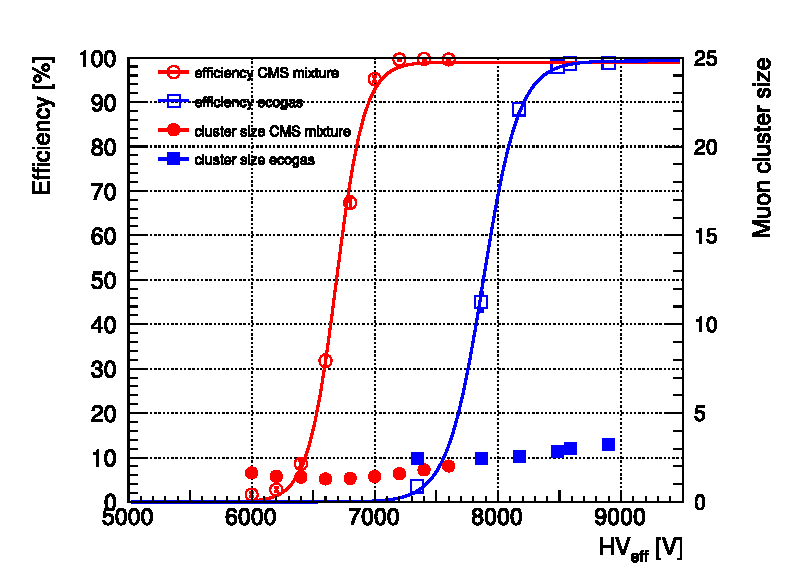
\includegraphics[width=\linewidth]{fig/chapt3/iRPC-HFO-mixture.pdf}
		\caption{\label{fig:iRPC-eco} Efficiency (open symbols) and cluster size (full symbols) of an iRPC as a function of the effective voltage for the standard CMS gas mixture and an environmental-friendly gas mixture.~\cite{PHASEIITP}.}
	\end{wrapfigure}
	
	Although the technology certification was conducted with the standard CMS gas mixture which is a known reference, the iRPCs will need to be operated with new environmental-friendly gas mixtures. Studies have then been conducted with iRPCs, assuming that the $HFO$/$CO_2$ mixture containing an almost equal level of both components was the most likely candidate to replace the standard mixture. In this purpose, an iRPC prototype has been built to be tested with an $HFO$/$CO_2$ gas mixture. The mixture, referred to as \textit{"ecogas"} in Figure~\ref{fig:iRPC-eco}, contained 50\% of $HFO$, 4.5\% of $iC_4H_{10}$, 0.3\% of $SF_6$ and 45.2\% of $CO_2$. In Figure~\ref{fig:iRPC-eco} is presented a result consistent with the blue curve obtained with 45\% of $HFO$, 4\% of $iC_4H_{10}$, 1\% of $SF_6$ and 50\% of $CO_2$ flushed into a standard double-gap RPC. Instead of the streamer probability, the cluster size is shown. The average number of hits generated by a muon passing through the chamber seem to have increased by 1 at the level of the knee of the sigmoid plateau using the ecogas.
	
\endgroup

\clearpage{\pagestyle{empty}\cleardoublepage}